\chapter{Modelo de madurez}
\label{ch:modelo-madurez}

El modelo de madurez es el componente del marco LLM-Sec que asigna a un sistema RAG un nivel en una escala ordinal según la solidez de sus controles de seguridad. Su construcción sigue tres pasos: la identificación de los activos de información que el sistema expone, la valoración del riesgo asociado a cada uno, y la definición de las subdimensiones y niveles sobre los cuales se realiza la evaluación. Las dos primeras secciones establecen el perímetro y la priorización; las restantes especifican la estructura del modelo, los seis niveles de madurez, las cinco subdimensiones y la regla de agregación del nivel global.


\section{Identificación de activos de información del sistema RAG}
\label{sec:activos}

Toda evaluación de seguridad requiere, como paso previo a la definición de controles, la identificación de los activos de información sobre los cuales opera el riesgo. Esta práctica está establecida en el NIST CSF 2.0 \cite{nistcsf}, cuya función \textit{Identify} define la gestión de activos como condición necesaria antes de seleccionar e implementar medidas de protección. En consecuencia, esta sección declara los activos del sistema RAG que el marco LLM-Sec tiene por objeto proteger, delimitando el perímetro de evaluación sobre el cual se articulan los componentes del marco. En este documento, el término activos de información se emplea en el sentido amplio de la norma ISO/IEC 27002:2022 \cite{iso27002}, que comprende tanto la información misma como los componentes tecnológicos que la procesan, almacenan y transportan, distinguiéndolo así del concepto contable de activo.

A diferencia de un LLM aislado, los sistemas RAG exponen una superficie de ataque distribuida en múltiples componentes encadenados, cada uno de los cuales constituye un activo susceptible de ser comprometido de forma independiente. La Tabla~\ref{tab:activos} presenta los cinco activos identificados, su descripción funcional dentro del flujo RAG y el riesgo principal asociado a cada uno.

\begin{table}[H]
\centering
\caption{Activos del sistema RAG y riesgos asociados.}
\label{tab:activos}
\rowcolors{2}{llmsec-gray}{white}
\begin{tabularx}{\textwidth}{@{} c >{\hsize=0.85\hsize\raggedright\arraybackslash}X >{\hsize=1.45\hsize\raggedright\arraybackslash}X >{\hsize=0.70\hsize\raggedright\arraybackslash}X @{}}
  \toprule
  \textbf{ID} & \textbf{Activo} & \textbf{Riesgo principal} & \textbf{Referencia} \\
  \midrule
  A1 & LLM &
    Manipulación del comportamiento del modelo mediante inyección de instrucciones maliciosas en lenguaje natural. &
    LLM01 \\
  A2 & Base de datos vectorial &
    Recuperación no autorizada de fragmentos indexados e intoxicación del corpus mediante documentos maliciosos. &
    LLM08 \\
  A3 & Corpus de conocimiento &
    Exposición de información sensible contenida en los documentos indexados mediante consultas diseñadas para exfiltración. &
    LLM02 \\
  A4 & Canales de entrada y salida &
    Transporte de instrucciones maliciosas en la entrada y filtración de información del corpus o del prompt del sistema en la salida. &
    LLM01, LLM07 \\
  A5 & Mecanismos de acceso y sesión &
    Acceso no autorizado a información sensible por ausencia de control de identidad o segregación de permisos. &
    NIST AI RMF \cite{nistairmf} \\
  \bottomrule
\end{tabularx}
\end{table}

Cada activo ocupa una posición específica dentro del flujo de inferencia RAG, lo que determina qué vectores de amenaza le son aplicables y, en consecuencia, qué subdimensión del modelo de madurez lo cubre. Las subdimensiones D1 a D5 referidas en este mapeo se definen formalmente en la sección \ref{sec:subdimensiones}; se anticipan aquí únicamente para establecer la trazabilidad entre activos de información y estructura del modelo.

\begin{table}[H]
  \centering
  \caption{Mapeo de activos de información a subdimensiones y vectores de amenaza.}
  \label{tab:mapeo-activos-subdim}
  \begin{tabularx}{\textwidth}{@{} c l l l l @{}}  % 5 columnas, no 4
    \toprule
    \textbf{Activo} & \textbf{Criticidad} & \textbf{Subdimensión} & \textbf{Vectores} & \textbf{Nivel} \\
    \midrule
    A1 (LLM)             & Crítico (25) & D1, D3 & 17 + 9 & Máxima \\
    A4 (Canales E/S)     & Crítico (20) & D1, D3 & 17 + 9 & Máxima \\
    A3 (Corpus)           & Alto (16) & D2     & 20      & Alta \\
    A2 (Base vectorial)   & Alto (15) & D2     & 20      & Alta \\
    A5 (Acceso y sesión)  & Bajo (4) & D4, D5 & 9 + 15 & Baja \\
    \bottomrule
  \end{tabularx}
\end{table}

\vspace{6pt}

Este mapeo justifica la existencia de exactamente cinco subdimensiones y no un número arbitrario: cada subdimensión protege un subconjunto distinto del flujo RAG, y el modelo de madurez evalúa cada uno de forma independiente antes de agregar un nivel global mediante la regla de piso mínimo (sección~\ref{sec:piso-minimo}).

\section{Valoración de riesgo por activo}
\label{sec:valoracion-riesgo}

La valoración emplea la matriz de riesgo de cinco por cinco descrita en la sección anterior, sobre la cual se definen cuatro zonas de clasificación (Bajo, Medio, Alto y Crítico) a partir del producto de probabilidad e impacto. La distribución resultante de los cinco activos revela una polarización característica de las arquitecturas RAG, que condiciona el diseño del modelo de madurez y la distribución de controles:

\begin{enumerate}[leftmargin=2em]
  \item \textbf{El LLM y los canales de entrada/salida presentan riesgo crítico.} Ambos activos combinan la máxima probabilidad de explotación con el mayor impacto, porque los vectores LLM01 y LLM07 son explotables con herramientas automatizadas de acceso público (como Garak \cite{garak}), sin requerir acceso privilegiado. La evidencia empírica respalda esta valoración: una revisión sistemática de 128 estudios reporta tasas de éxito de inyección superiores al 90\% contra sistemas sin protección \cite{promptinjsurvey}. El compromiso del LLM implica además la pérdida de control sobre el comportamiento del modelo, el impacto de mayor severidad del sistema. Esta condición explica que las subdimensiones que interceptan estos vectores concentren la mayor densidad de controles técnicos: D1 (Protección de entrada) agrupa 17 controles y D2 (Control de contexto y configuración RAG) agrupa 20, los dos volúmenes más altos del marco. D3 (Gestión de salida) los complementa con 9 controles sobre un único canal, el de respuesta.
  \item \textbf{El corpus y la base vectorial presentan riesgo alto.} El corpus es exfiltrable mediante consultas diseñadas (LLM02), mientras que la base vectorial exige condiciones que un atacante externo no posee por defecto: capacidad de escritura sobre la base de conocimiento y conocimiento específico de la infraestructura de recuperación. No obstante, su impacto es muy alto: se ha demostrado que la inyección de apenas cinco textos maliciosos por pregunta objetivo alcanza un 90\% de éxito en corromper las respuestas de un sistema RAG, incluso sobre bases con millones de fragmentos \cite{poisonedrag}. Esto justifica que D2 sea la subdimensión con mayor densidad de controles (20).
  \item \textbf{Los mecanismos de acceso y sesión presentan riesgo bajo.} Su probabilidad de explotación es la mínima de la escala porque su compromiso exige condiciones poco frecuentes: la posesión de credenciales privilegiadas válidas, sea por compromiso externo o por posición interna, o una falla de configuración en la capa de identidad. El informe de brechas de Verizon, sobre más de 12.000 brechas confirmadas, muestra que los actores internos originan una fracción minoritaria de ellas, con un 5\% en Norteamérica y un máximo regional de 29\% en EMEA, del cual solo un 8\% corresponde a uso indebido de privilegios \cite{dbir2025}. Su impacto, en cambio, permanece alto. Esto justifica que el control de acceso por sesión (C22) se clasifique con fuente de evidencia declarativa: su verificación depende de la capa de identidad y autenticación de la organización, componente externo al flujo de inferencia RAG y por tanto no evaluable mediante auditoría ofensiva contra el sistema. Su implementación sigue siendo imprescindible en todo despliegue productivo.
\end{enumerate}

La zona de riesgo Medio no contiene activos. Lejos de ser una deficiencia de la valoración, esta ausencia refleja la naturaleza polarizada de la superficie de ataque de un sistema RAG: sus activos son atacables con herramientas de acceso público, y por tanto de riesgo alto o crítico, o bien exigen condiciones de acceso privilegiado que reducen su probabilidad a la mínima de la escala, situándolos en riesgo bajo pese a su impacto elevado. El instrumento discrimina así entre dos regímenes de amenaza cualitativamente distintos, que demandan estrategias de control diferenciadas.

\subsection{Escala de valoración}

La valoración emplea dos ejes de cinco niveles cada uno: probabilidad de explotación e impacto de compromiso. La Tabla~\ref{tab:escala-prob} describe la escala de probabilidad de explotación.

\begin{table}[H]
  \centering
  \caption{Escala de valoración de probabilidad de explotación.}
  \label{tab:escala-prob}
  \begin{tabularx}{\textwidth}{@{} c l >{\raggedright\arraybackslash}X @{}}
    \toprule
    \textbf{Nivel} & \textbf{Etiqueta} & \textbf{Descripción} \\
    \midrule
    5 & Muy alta & Explotable con herramientas automatizadas de acceso público, sin conocimiento del sistema ni acceso privilegiado; éxito demostrado superior al 90\% contra sistemas sin protección. \\
    4 & Alta     & Explotable con herramientas de acceso público que requieren configuración o adaptación menor al objetivo. \\
    3 & Media    & Requiere conocimiento técnico específico de la infraestructura del sistema, como el tipo de base vectorial o la estrategia de indexación. \\
    2 & Baja     & Requiere capacidad de escritura sobre componentes internos o conocimiento no público de la configuración. \\
    1 & Muy baja & Requiere la posesión de credenciales privilegiadas válidas o una condición de configuración poco frecuente. \\
    \bottomrule
  \end{tabularx}
\end{table}

La Tabla~\ref{tab:escala-impacto} describe la escala de impacto de compromiso.

\begin{table}[H]
  \centering
  \caption{Escala de valoración de impacto de compromiso.}
  \label{tab:escala-impacto}
  \begin{tabularx}{\textwidth}{@{} c l >{\raggedright\arraybackslash}X @{}}
    \toprule
    \textbf{Nivel} & \textbf{Etiqueta} & \textbf{Descripción} \\
    \midrule
    5 & Muy alto & Pérdida de control sobre el comportamiento del modelo o exfiltración masiva de datos sensibles del corpus. \\
    4 & Alto     & Exfiltración puntual de información sensible o compromiso de la integridad del corpus recuperable. \\
    3 & Medio    & Exposición parcial de información o degradación del servicio. \\
    2 & Bajo     & Impacto operacional contenido, sin exposición de datos. \\
    1 & Muy bajo & Efecto marginal, sin consecuencia sobre datos ni disponibilidad. \\
    \bottomrule
  \end{tabularx}
\end{table}

\subsection{Matriz de riesgo}

% Colores de las cuatro zonas de clasificación de riesgo
\definecolor{riesgo-bajo}{HTML}{4CAF7D}
\definecolor{riesgo-medio}{HTML}{E8B93D}
\definecolor{riesgo-alto}{HTML}{E8792F}
\definecolor{riesgo-critico}{HTML}{D64545}

La Tabla~\ref{tab:matriz-riesgo} presenta la valoración de riesgo para cada activo identificado en la sección anterior. El nivel de riesgo se obtiene como el producto de probabilidad e impacto, clasificado en cuatro zonas conforme a la metodología de valoración de riesgo de NIST SP 800-30 \cite{nist80030}: \textbf{Bajo} ($1$--$4$), \textbf{Medio} ($5$--$9$), \textbf{Alto} ($10$--$16$) y \textbf{Crítico} ($17$--$25$).

\begin{table}[H]
\centering
\caption{Matriz de valoración de riesgo por activo del sistema RAG.}
\label{tab:matriz-riesgo}
\begin{tabularx}{\textwidth}{@{} c l C{2.5cm} C{2.5cm} C{1.8cm} C{2cm} @{}}
  \toprule
  \textbf{ID} & \textbf{Activo} & \textbf{Probabilidad} & \textbf{Impacto} & \textbf{Producto} & \textbf{Zona} \\
  \midrule
  A1 & LLM                   & 5 (Muy alta) & 5 (Muy alto) & 25 & \badge{riesgo-critico}{Crítico} \\[4pt]
  A4 & Canales de E/S        & 5 (Muy alta) & 4 (Alto)     & 20 & \badge{riesgo-critico}{Crítico} \\[4pt]
  A3 & Corpus                & 4 (Alta)     & 4 (Alto)     & 16 & \badge{riesgo-alto}{Alto} \\[4pt]
  A2 & Base vectorial        & 3 (Media)    & 5 (Muy alto) & 15 & \badge{riesgo-alto}{Alto} \\[4pt]
  A5 & Acceso y sesión       & 1 (Muy baja) & 4 (Alto)     &  4 & \badge{riesgo-bajo}{Bajo} \\
  \bottomrule
\end{tabularx}
\end{table}

La Figura~\ref{fig:matriz-visual} ubica cada activo en la matriz probabilidad $\times$ impacto, evidenciando la concentración del riesgo en la zona superior derecha.

\begin{figure}[H]
\centering
\begin{tikzpicture}[
  cell/.style={
    minimum width=2.3cm, minimum height=1.75cm,
    draw=white, line width=1.5pt,
    align=center, font=\scriptsize\bfseries
  },
  axislabel/.style={font=\small\bfseries, text=llmsec-dark},
  ticklabel/.style={font=\scriptsize, text=llmsec-dark},
  legendlabel/.style={font=\scriptsize, text=llmsec-dark},
  activo/.style={font=\scriptsize\bfseries, text=white}
]

% Fila Impacto = 5 (Muy alto)
\node[cell, fill=riesgo-medio,   text=white] at (0,7.6)   {5\\[-2pt]\tiny Medio};
\node[cell, fill=riesgo-alto,    text=white] at (2.4,7.6) {10\\[-2pt]\tiny Alto};
\node[cell, fill=riesgo-alto,    text=white] at (4.8,7.6) {15\\[-2pt]\tiny Alto};
\node[cell, fill=riesgo-critico, text=white] at (7.2,7.6) {20\\[-2pt]\tiny Crítico};
\node[cell, fill=riesgo-critico, text=white] at (9.6,7.6) {25\\[-2pt]\tiny Crítico};

% Fila Impacto = 4 (Alto)
\node[cell, fill=riesgo-bajo,    text=white] at (0,5.7)   {4\\[-2pt]\tiny Bajo};
\node[cell, fill=riesgo-medio,   text=white] at (2.4,5.7) {8\\[-2pt]\tiny Medio};
\node[cell, fill=riesgo-alto,    text=white] at (4.8,5.7) {12\\[-2pt]\tiny Alto};
\node[cell, fill=riesgo-alto,    text=white] at (7.2,5.7) {16\\[-2pt]\tiny Alto};
\node[cell, fill=riesgo-critico, text=white] at (9.6,5.7) {20\\[-2pt]\tiny Crítico};

% Fila Impacto = 3 (Medio)
\node[cell, fill=riesgo-bajo,    text=white] at (0,3.8)   {3\\[-2pt]\tiny Bajo};
\node[cell, fill=riesgo-medio,   text=white] at (2.4,3.8) {6\\[-2pt]\tiny Medio};
\node[cell, fill=riesgo-medio,   text=white] at (4.8,3.8) {9\\[-2pt]\tiny Medio};
\node[cell, fill=riesgo-alto,    text=white] at (7.2,3.8) {12\\[-2pt]\tiny Alto};
\node[cell, fill=riesgo-alto,    text=white] at (9.6,3.8) {15\\[-2pt]\tiny Alto};

% Fila Impacto = 2 (Bajo)
\node[cell, fill=riesgo-bajo,    text=white] at (0,1.9)   {2\\[-2pt]\tiny Bajo};
\node[cell, fill=riesgo-bajo,    text=white] at (2.4,1.9) {4\\[-2pt]\tiny Bajo};
\node[cell, fill=riesgo-medio,   text=white] at (4.8,1.9) {6\\[-2pt]\tiny Medio};
\node[cell, fill=riesgo-medio,   text=white] at (7.2,1.9) {8\\[-2pt]\tiny Medio};
\node[cell, fill=riesgo-alto,    text=white] at (9.6,1.9) {10\\[-2pt]\tiny Alto};

% Fila Impacto = 1 (Muy bajo)
\node[cell, fill=riesgo-bajo,    text=white] at (0,0)     {1\\[-2pt]\tiny Bajo};
\node[cell, fill=riesgo-bajo,    text=white] at (2.4,0)   {2\\[-2pt]\tiny Bajo};
\node[cell, fill=riesgo-bajo,    text=white] at (4.8,0)   {3\\[-2pt]\tiny Bajo};
\node[cell, fill=riesgo-bajo,    text=white] at (7.2,0)   {4\\[-2pt]\tiny Bajo};
\node[cell, fill=riesgo-medio,   text=white] at (9.6,0)   {5\\[-2pt]\tiny Medio};

% Activos ubicados (probabilidad, impacto)
\node[activo] at (9.6,8.15) {A1};
\node[activo] at (9.6,6.25) {A4};
\node[activo] at (7.2,6.25) {A3};
\node[activo] at (4.8,8.15) {A2};
\node[activo] at (0,6.25)   {A5};

% Etiquetas de eje X (probabilidad)
\node[ticklabel] at (0,-1.2)   {1 (Muy baja)};
\node[ticklabel] at (2.4,-1.2) {2 (Baja)};
\node[ticklabel] at (4.8,-1.2) {3 (Media)};
\node[ticklabel] at (7.2,-1.2) {4 (Alta)};
\node[ticklabel] at (9.6,-1.2) {5 (Muy alta)};
\node[axislabel] at (4.8,-1.8) {Probabilidad de explotación};

% Etiquetas de eje Y (impacto)
\node[ticklabel, rotate=90] at (-2.0,7.6) {5 (Muy alto)};
\node[ticklabel, rotate=90] at (-2.0,5.7) {4 (Alto)};
\node[ticklabel, rotate=90] at (-2.0,3.8) {3 (Medio)};
\node[ticklabel, rotate=90] at (-2.0,1.9) {2 (Bajo)};
\node[ticklabel, rotate=90] at (-2.0,0)   {1 (Muy bajo)};
\node[axislabel, rotate=90] at (-2.6,3.8) {Impacto de compromiso};

% Leyenda de zonas
\node[fill=riesgo-bajo,    minimum width=0.35cm, minimum height=0.35cm, draw=none] at (0,-2.8)   {};
\node[legendlabel, anchor=west] at (0.25,-2.8)   {Bajo};
\node[fill=riesgo-medio,   minimum width=0.35cm, minimum height=0.35cm, draw=none] at (2.7,-2.8) {};
\node[legendlabel, anchor=west] at (2.95,-2.8)   {Medio};
\node[fill=riesgo-alto,    minimum width=0.35cm, minimum height=0.35cm, draw=none] at (5.4,-2.8) {};
\node[legendlabel, anchor=west] at (5.65,-2.8)   {Alto};
\node[fill=riesgo-critico, minimum width=0.35cm, minimum height=0.35cm, draw=none] at (8.0,-2.8) {};
\node[legendlabel, anchor=west] at (8.25,-2.8)   {Crítico};

\end{tikzpicture}
\caption{Matriz de riesgo probabilidad $\times$ impacto con la ubicación de los activos del sistema RAG.}
\label{fig:matriz-visual}
\end{figure}

\subsection{Trazabilidad hacia las subdimensiones}

La valoración de riesgo justifica la estructura del modelo de madurez de la siguiente forma:

\begin{table}[H]
  \centering
  \caption{Trazabilidad entre riesgo valorado y densidad de controles.}
  \label{tab:trazabilidad-riesgo}
  \begin{tabularx}{\textwidth}{@{} c l c c c @{}}
    \toprule
    \textbf{Activo} & \textbf{Riesgo} & \textbf{Subdimensión} & \textbf{Controles} & \textbf{Prioridad} \\
    \midrule
    A1 (LLM)             & Crítico (25) & D1, D3 & 17 + 9 & Máxima \\
    A4 (Canales E/S)     & Crítico (20) & D1, D3 & 17 + 9 & Máxima \\
    A3 (Corpus)           & Alto (16) & D2     & 20      & Alta \\
    A2 (Base vectorial)   & Alto (15) & D2     & 20      & Alta \\
    A5 (Acceso y sesión)  & Bajo (4) & D4, D5 & 9 + 15 & Baja \\
    \bottomrule
  \end{tabularx}
\end{table}

\vspace{6pt}

Esta trazabilidad garantiza que la distribución de controles del marco no es arbitraria: en las subdimensiones técnicas, la densidad de controles es proporcional al riesgo valorado de los activos que protegen, con D1 y D2, asociadas a los activos de riesgo crítico y alto, concentrando los mayores volúmenes. D4, de naturaleza observacional, y D5, cuya densidad responde a las obligaciones normativas ancladas en la Ley 21.663 y la Ley 21.719 más que al riesgo técnico de un activo específico, completan la cobertura priorizando la observación y la gobernanza sobre la intervención directa. El activo de riesgo bajo (A5) se cubre mediante un control declarativo, coherente con su naturaleza externa al flujo de inferencia. Los controles transversales se contabilizan en cada subdimensión a la que pertenecen, por lo que la suma de aplicaciones (70) excede el total de controles únicos del marco (62), conforme al criterio declarado en el Capítulo~\ref{ch:controles}.

\begin{infobox}
  La valoración presentada corresponde a un sistema RAG genérico. Cada organización debe recalcular la probabilidad y el impacto según su contexto de despliegue específico, utilizando las escalas definidas en las Tablas~\ref{tab:escala-prob} y~\ref{tab:escala-impacto}. El perfil organizacional (P1, P2 o P3) orienta la interpretación del nivel de riesgo aceptable, pero no reemplaza esta valoración.
\end{infobox}

\section{Estructura del modelo}

A partir de los activos de información identificados y su valoración de riesgo (secciones~\ref{sec:activos} y~\ref{sec:valoracion-riesgo}), el modelo de madurez LLM-Sec define seis niveles (N0 a N5) que representan una escala ordinal de la postura de ciberseguridad de un sistema RAG, conforme a los conceptos de evaluación de procesos de ISO/IEC 33001 \cite{iso33001}. La progresión es acumulativa: alcanzar un nivel $N_k$ requiere satisfacer todos los criterios de los niveles $N_1$ a $N_{k}$. Las distancias entre niveles no son uniformes; cada nivel refleja un salto cualitativo en la solidez de los procesos, no un incremento lineal.

El modelo evalúa cinco subdimensiones derivadas de los ítems del OWASP LLM Top 10:2025 \cite{owasp2025} pertinentes al flujo RAG, cuya trazabilidad hacia los activos del sistema se estableció en la sección~\ref{sec:activos}. Dado que no existe un modelo de madurez ordinal con progresión acumulativa y validación experimental para arquitecturas RAG en la literatura ni en los estándares actuales, esta derivación constituye una contribución original del marco.

\section{Niveles de madurez}

\begin{levelbox}[title=N0: No conforme]{level-n0}
  El sistema incumple al menos un control de nivel N1 en alguna subdimensión aplicable, operando sin las salvaguardas mínimas exigibles. Corresponde a un sistema RAG desplegado sin capa defensiva o con controles básicos ausentes. No constituye un nivel de madurez, sino el estado de no conformidad con el marco.
\end{levelbox}
\vspace{8pt}

\begin{levelbox}[title=N1: Inicial]{level-n1}
  Controles preventivos básicos de nivel N1 implementados en todas las subdimensiones aplicables: restricciones de entrada, delimitación del contexto inyectado y prompt del sistema con instrucciones de seguridad, con la capa defensiva activa en configuración por defecto. La protección es estática: no existe calibración de umbrales, monitoreo ni respuesta ante incidentes.
\end{levelbox}

\vspace{8pt}

\begin{levelbox}[title=N2: Reactivo]{level-n2}
  Umbrales de detección configurados y logging básico habilitado. La organización responde ante incidentes conocidos, pero la operación de seguridad no es preventiva ni está formalmente documentada. La tasa de filtrado de ataques es positiva pero variable entre categorías de amenaza.
\end{levelbox}

\vspace{8pt}

\begin{levelbox}[title=N3: Definido]{level-n3}
  Controles formalmente definidos, documentados y aplicados de forma consistente. Umbrales de detección establecidos antes de la operación. Los logs de la capa defensiva son trazables por escáner y categoría de amenaza.
\end{levelbox}

\vspace{8pt}

\begin{levelbox}[title=N4: Gestionado]{level-n4}
  Seguridad gestionada cuantitativamente. Métricas de desempeño definidas (TFA, LAS, PCC, NCP) y controles ajustados según resultados medidos. La consistencia de la protección entre categorías de amenaza se evalúa periódicamente mediante el indicador NCP.
\end{levelbox}

\vspace{8pt}

\begin{levelbox}[title=N5: Optimizado]{level-n5}
  Mejora continua. Controles actualizados proactivamente ante nuevas amenazas documentadas. Marco revisado periódicamente e integrado al ciclo de gestión de riesgos organizacional.
\end{levelbox}

La estructura del modelo se alinea con los modelos de madurez consolidados en la industria. Al igual que CMMI \cite{cmmi} e ISO/IEC 33020 \cite{iso33020}, LLM-Sec emplea una escala ordinal de niveles cualitativos con progresión acumulativa, donde cada nivel presupone la satisfacción de los anteriores. El nivel N0 cumple la función del nivel 0 (\textit{Incomplete}) de ISO/IEC 33020: un estado fuera de la escala de madurez propiamente tal, que señala la ausencia de las condiciones mínimas de evaluación. La correspondencia más directa se da en N4: su definición por gestión cuantitativa mediante métricas coincide con el nivel \textit{Quantitatively Managed} de CMMI, definido por el control estadístico y cuantitativo de los procesos. No se presenta un mapeo exhaustivo nivel a nivel porque los dominios de definición difieren: los niveles de CMMI se articulan sobre áreas de proceso del desarrollo de software, mientras que los de LLM-Sec se articulan sobre controles de ciberseguridad específicos del flujo RAG, de modo que la equivalencia entre ambos modelos es estructural y no semántica.

\section{Subdimensiones}
\label{sec:subdimensiones}

El modelo organiza la evaluación en cinco subdimensiones, cada una derivada de los vectores de amenaza del OWASP LLM Top 10:2025 \cite{owasp2025} pertinentes al flujo RAG. Las tres primeras (D1, D2, D3) operan sobre etapas específicas del flujo de inferencia: entrada, recuperación y salida respectivamente. D4 opera de forma transversal registrando los eventos generados por las anteriores, y D5 captura las obligaciones organizacionales que sustentan la operación segura del sistema en su conjunto. Esta estructura garantiza que cada punto del flujo RAG identificado en la sección~\ref{sec:activos} sea cubierto por al menos una subdimensión, y que la densidad de controles de cada una sea proporcional al riesgo valorado en la sección~\ref{sec:valoracion-riesgo}. Los vectores OWASP asociados a cada subdimensión corresponden a los que sus controles abordan de forma principal; controles individuales, en particular los transversales, pueden referenciar adicionalmente otros vectores en su fuente, lo que se detalla en la taxonomía del Capítulo~\ref{ch:controles}. 

El OWASP LLM Top 10:2025 cumple en este marco la función de catálogo de referencia de amenazas: enumera y caracteriza los vectores de ataque, pero no prescribe cómo verificar su mitigación ni cómo medir la madurez de los controles que los abordan. Estas funciones corresponden a otros instrumentos del mismo ecosistema OWASP. El AISVS \cite{aisvs} aporta la capa de verificación, especificando requisitos comprobables para cada familia de controles, y LLM-Sec aporta la capa de madurez, situando la postura de seguridad en una escala ordinal validada experimentalmente. Los tres instrumentos son complementarios y operan sobre planos distintos del mismo problema: el Top 10 describe qué puede fallar, AISVS qué debe verificarse y LLM-Sec cuán maduro es el proceso que lo gestiona. El marco LLM-Sec adopta el Top 10:2025 como fuente normativa de los vectores que sus subdimensiones cubren, y su relación con AISVS se detalla en la sección~\ref{sec:relacion-aisvs}.

La Tabla~\ref{tab:subdimensiones} sintetiza las cinco subdimensiones, los vectores OWASP que cubre cada una y el aspecto del sistema que captura. 

\begin{table}[H]
  \centering
  \caption{Subdimensiones del modelo LLM-Sec.}
  \label{tab:subdimensiones}
  \begin{tabularx}{\textwidth}{@{}c l l X@{}}
    \toprule
    \textbf{ID} & \textbf{Nombre} & \textbf{OWASP} & \textbf{Captura} \\
    \midrule
    D1 & Protección de entrada    & LLM01, LLM02     & Validación y sanitización de prompts \\
    D2 & Control de contexto y configuración RAG  & LLM02, LLM08 & Acceso y exposición de la base vectorial \\
    D3 & Gestión de salida        & LLM02, LLM07 & Filtrado y control de respuestas \\
    D4 & Monitoreo y trazabilidad & Todos         & Logging, alertas y auditoría \\
    D5 & Gobernanza organizacional & ---           & Roles, políticas y cultura de seguridad \\
    \bottomrule
  \end{tabularx}
\end{table}

\begin{figure}[H]
  \centering
  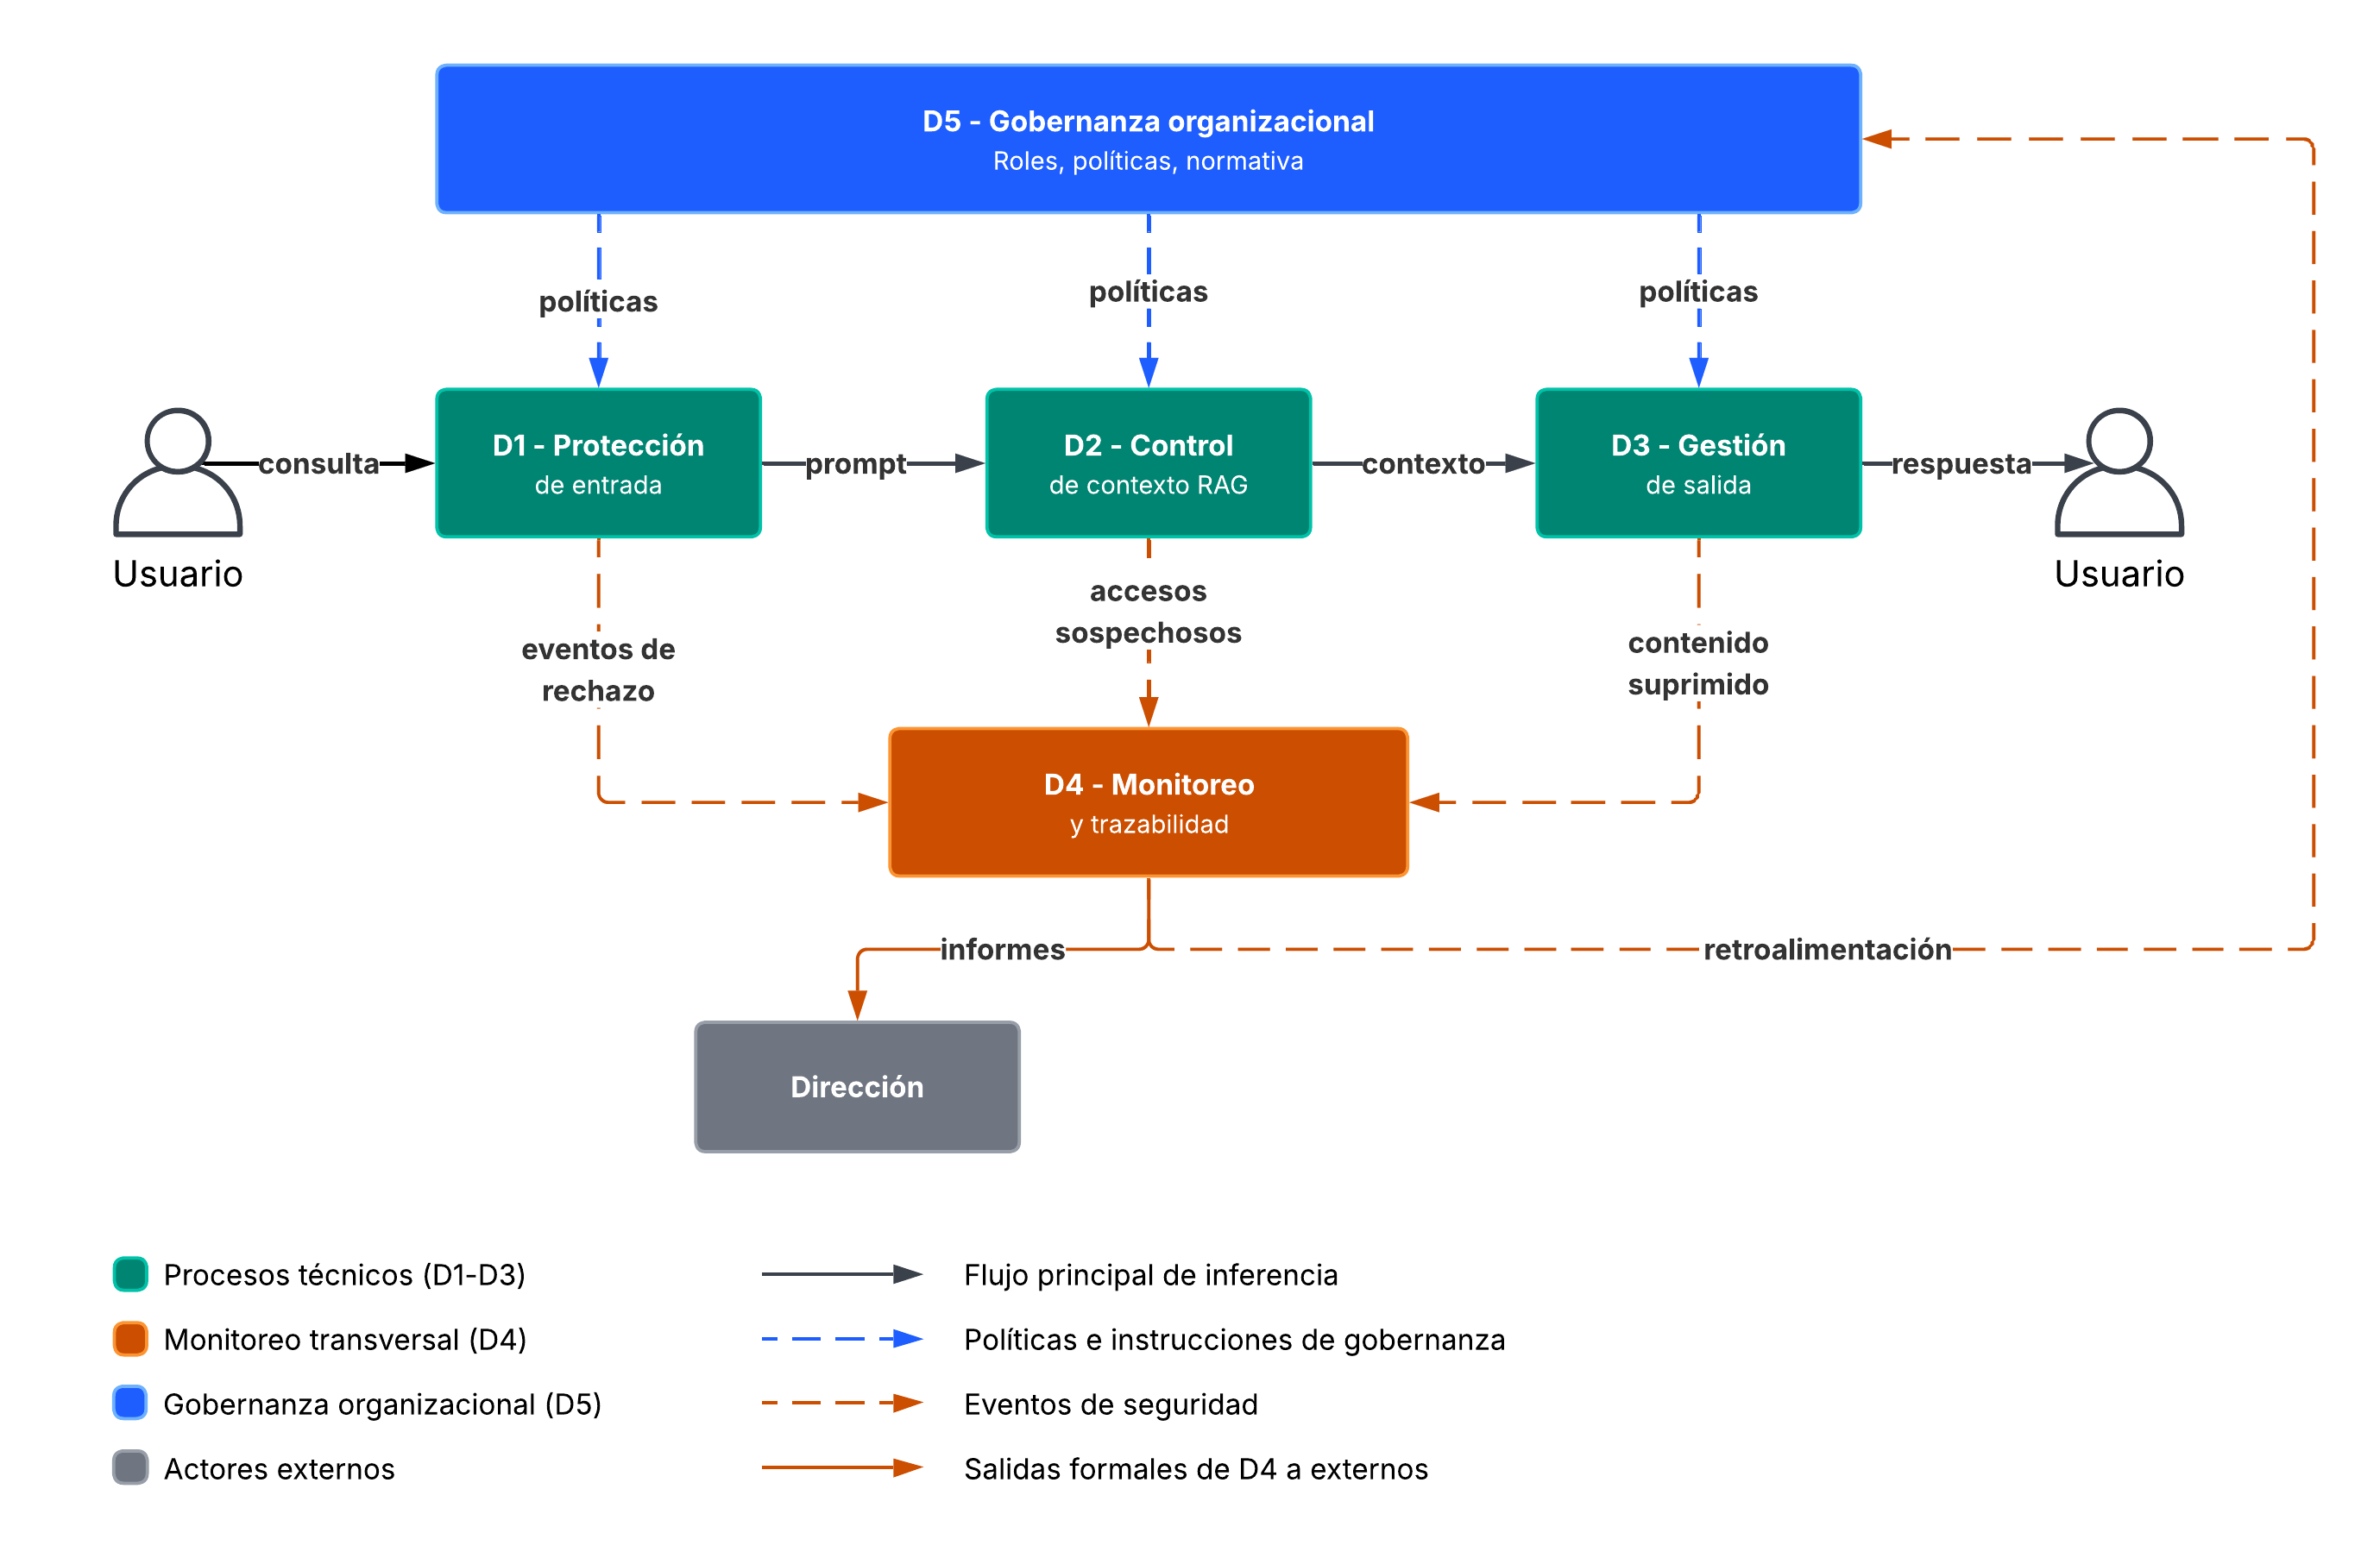
\includegraphics[width=0.95\linewidth]{figures/es_general.png}
  \caption{Flujo de entradas y salidas de todos los procesos.}
  \label{fig:diagrama-general}
\end{figure}

\subsection{D1: Protección de entrada}

La subdimensión D1 representa el primer punto de contacto entre el usuario y el sistema RAG, constituyendo la primera línea de defensa para garantizar una secuencia de acciones segura. Los activos de información sobre los que opera son los canales de entrada y el propio LLM, cuyo comportamiento puede ser manipulado si el prompt no es validado previamente.

La ficha del proceso y su especificación de entradas y salidas se presentan a continuación; la Figura~\ref{fig:diagrama-d1} representa gráficamente el mismo flujo.

\begin{fichabox}{Ficha del proceso D1: Protección de entrada}
  \begin{tabularx}{\textwidth}{@{} l X @{}}
    \textbf{Propósito} &
      Interceptar amenazas semánticas antes de que alcancen la capa
      de inferencia, mediante validación y sanitización del prompt
      de entrada. \\[4pt]
    \textbf{Activos que protege} &
      Canales de entrada y LLM. \\[4pt]
    \textbf{Vector OWASP asociado} &
      LLM01:2025, LLM02:2025 \\
  \end{tabularx}
\end{fichabox}

\begin{table}[H]
  \centering
  \caption{Entradas y salidas del proceso D1: Protección de entrada.}
  \label{tab:es-d1}
  \rowcolors{2}{llmsec-gray}{white}
  \begin{tabularx}{\textwidth}{@{} l l X l @{}}
    \toprule
    \textbf{Desde} & \textbf{Entrada} &
    \textbf{Salida} & \textbf{Hacia} \\
    \midrule
    Usuario &
      Prompt en lenguaje natural &
      Prompt sanitizado y validado &
      D2 \\
    Sistema &
      System prompt configurado &
      Registro de prompts rechazados &
      D4 \\
    Configuración &
      Políticas de restricción (YAML) &
      Alerta de intento de inyección detectado &
      D4 \\
    D5 &
      Política de uso aceptable &
      --- &
      --- \\
    \bottomrule
  \end{tabularx}
\end{table}

\vspace{8pt}

\begin{figure}[H]
    \centering
    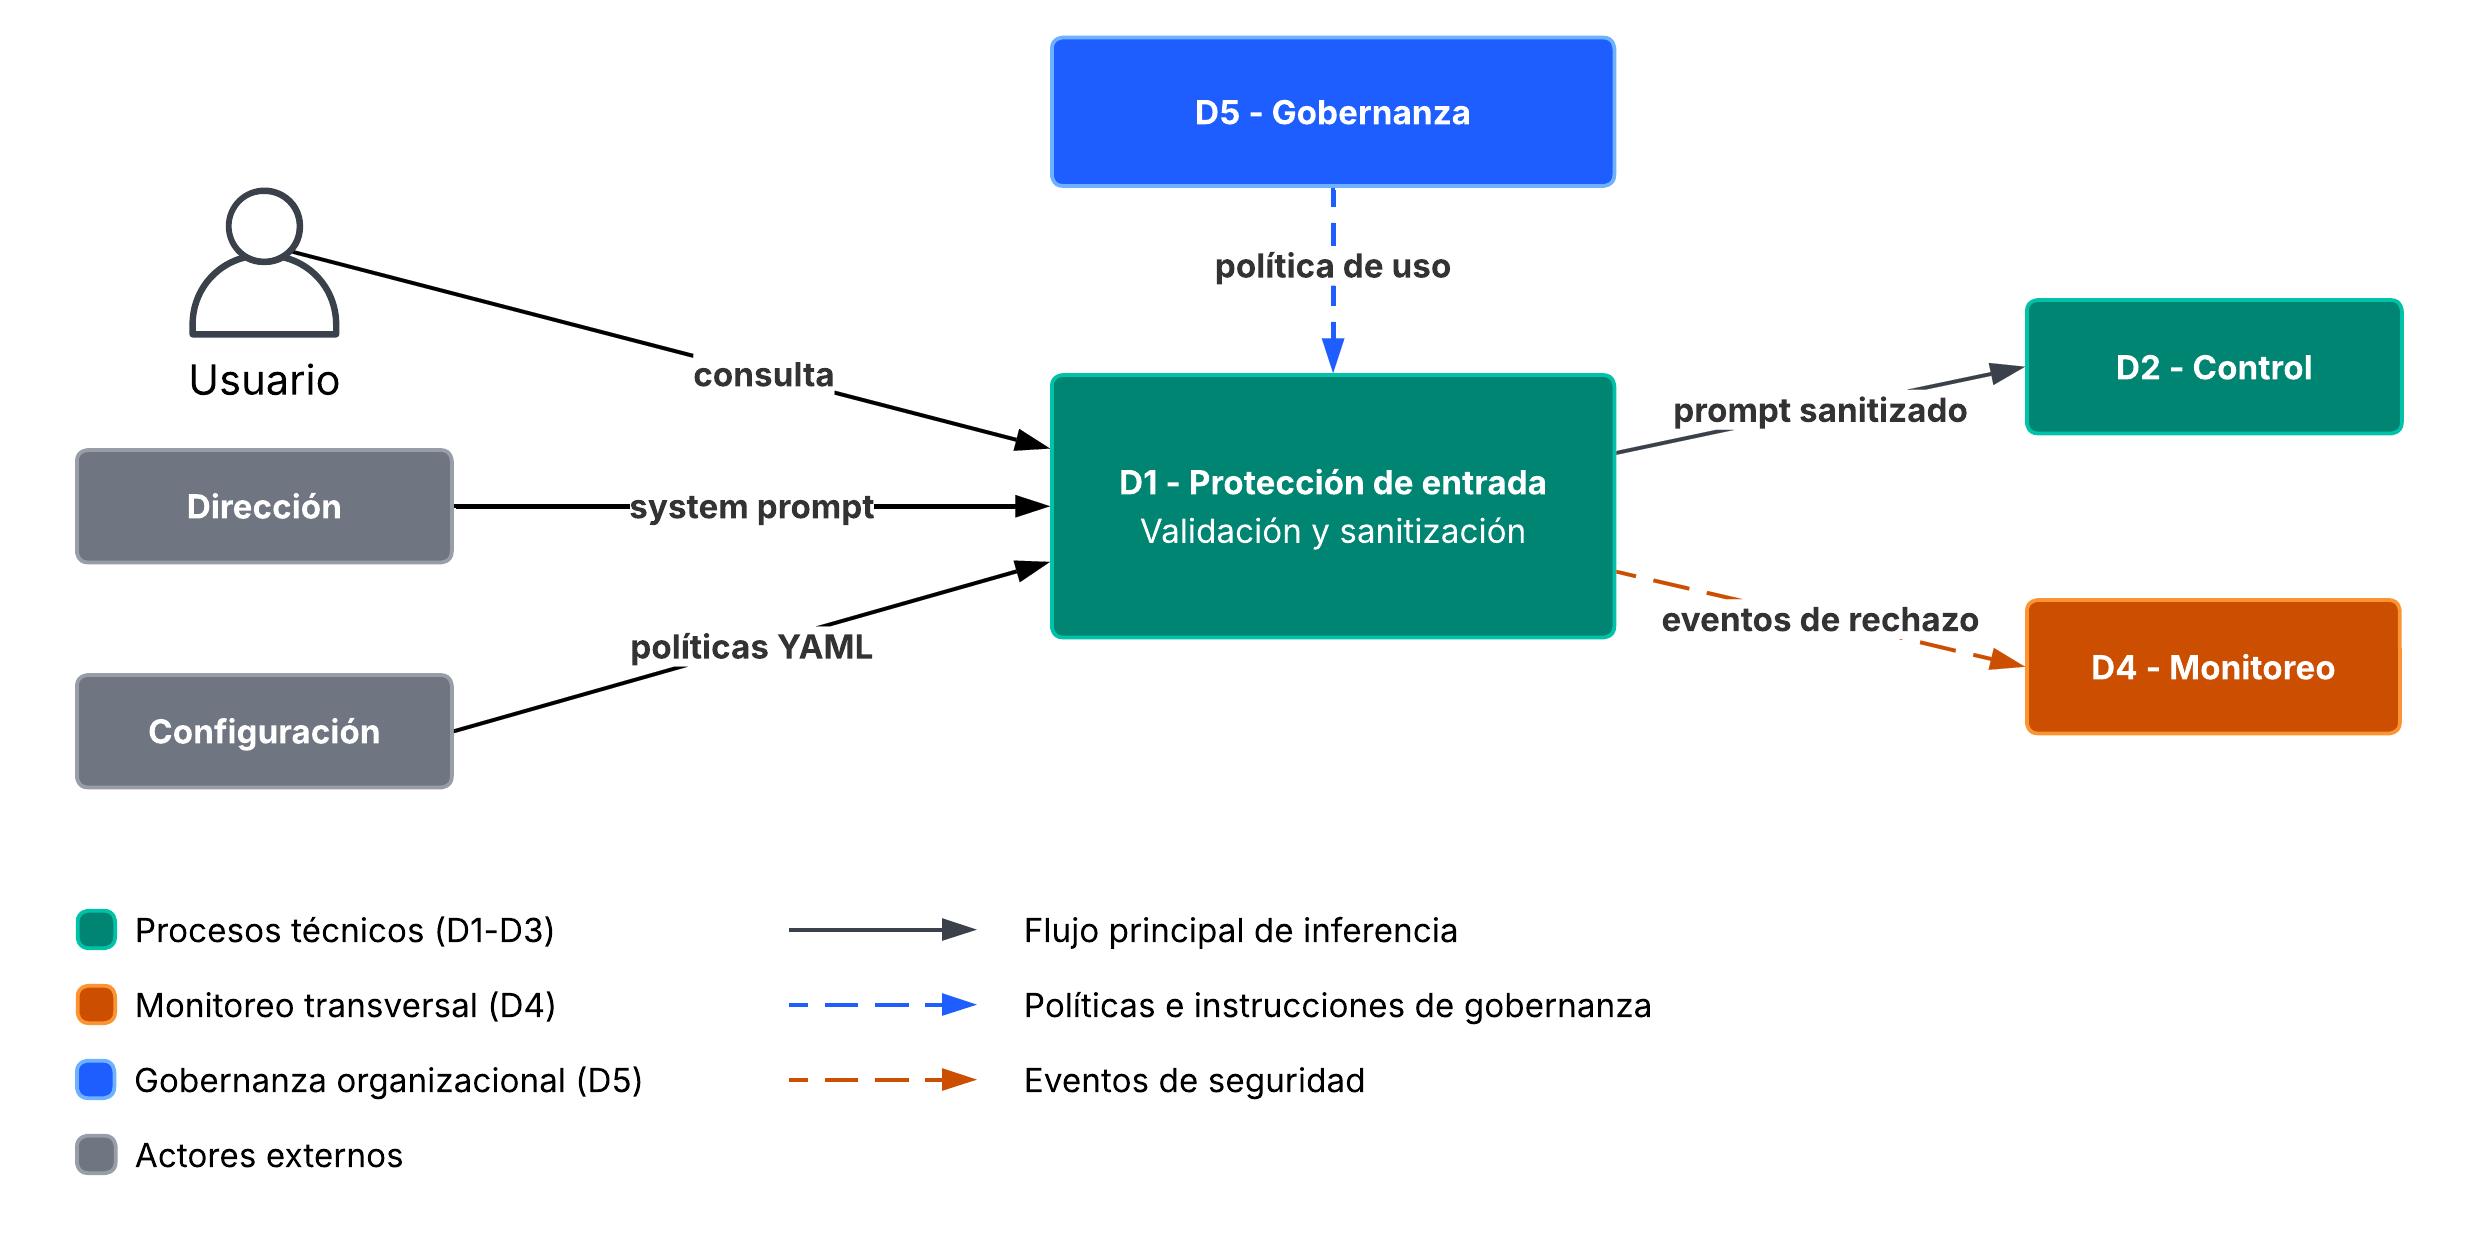
\includegraphics[width=0.95\linewidth]{figures/diagrama_D1.png}
    \caption{Flujo de entradas y salidas del proceso D1: Protección de entrada.}
    \label{fig:diagrama-d1}
\end{figure}

\subsection{D2: Control de contexto y configuración RAG}

La subdimensión D2 abarca los controles que regulan el acceso, la exposición y la integridad de la base de datos vectorial y el corpus de conocimiento. Opera sobre la etapa de recuperación del flujo RAG, donde los fragmentos de contexto son seleccionados y entregados al modelo como parte del prompt aumentado.

La ficha del proceso y su especificación de entradas y salidas se presentan a continuación; la Figura~\ref{fig:diagrama-d2} representa gráficamente el mismo flujo.

\begin{fichabox}{Ficha del proceso D2: Control de contexto y configuración RAG}
  \begin{tabularx}{\textwidth}{@{} l X @{}}
    \textbf{Propósito} &
      Controlar el acceso y la exposición del corpus indexado, limitando qué fragmentos pueden ser recuperados e incorporados al contexto de inferencia del LLM. \\[4pt]
    \textbf{Activos que protege} &
      Base de datos vectorial y corpus de conocimiento. \\[4pt]
    \textbf{Vector OWASP asociado} &
      LLM02:2025, LLM08:2025 \\
  \end{tabularx}
\end{fichabox}

\begin{table}[H]
  \centering
  \caption{Entradas y salidas del proceso D2: Control de contexto y configuración RAG.}
  \label{tab:es-d2}
  \rowcolors{2}{llmsec-gray}{white}
  \begin{tabularx}{\textwidth}{@{} l >{\hsize=1.10\hsize\raggedright\arraybackslash}X >{\hsize=0.90\hsize\raggedright\arraybackslash}X l @{}}
    \toprule
    \textbf{Desde} & \textbf{Entrada} & \textbf{Salida} & \textbf{Hacia} \\
    \midrule
    D1 &
      Prompt sanitizado y validado &
      Contexto recuperado y prompt aumentado &
      D3 \\
    Corpus &
      Documentos indexados &
      Contexto recuperado y prompt aumentado &
      D3 \\
    Sistema &
      Configuración del \textit{vector store} &
      Eventos de recuperación sospechosa &
      D4 \\
    D5 &
      Política de clasificación de sensibilidad del corpus &
      --- &
      --- \\
    \bottomrule
  \end{tabularx}
\end{table}

\vspace{8pt}

\begin{figure}[H]
    \centering
    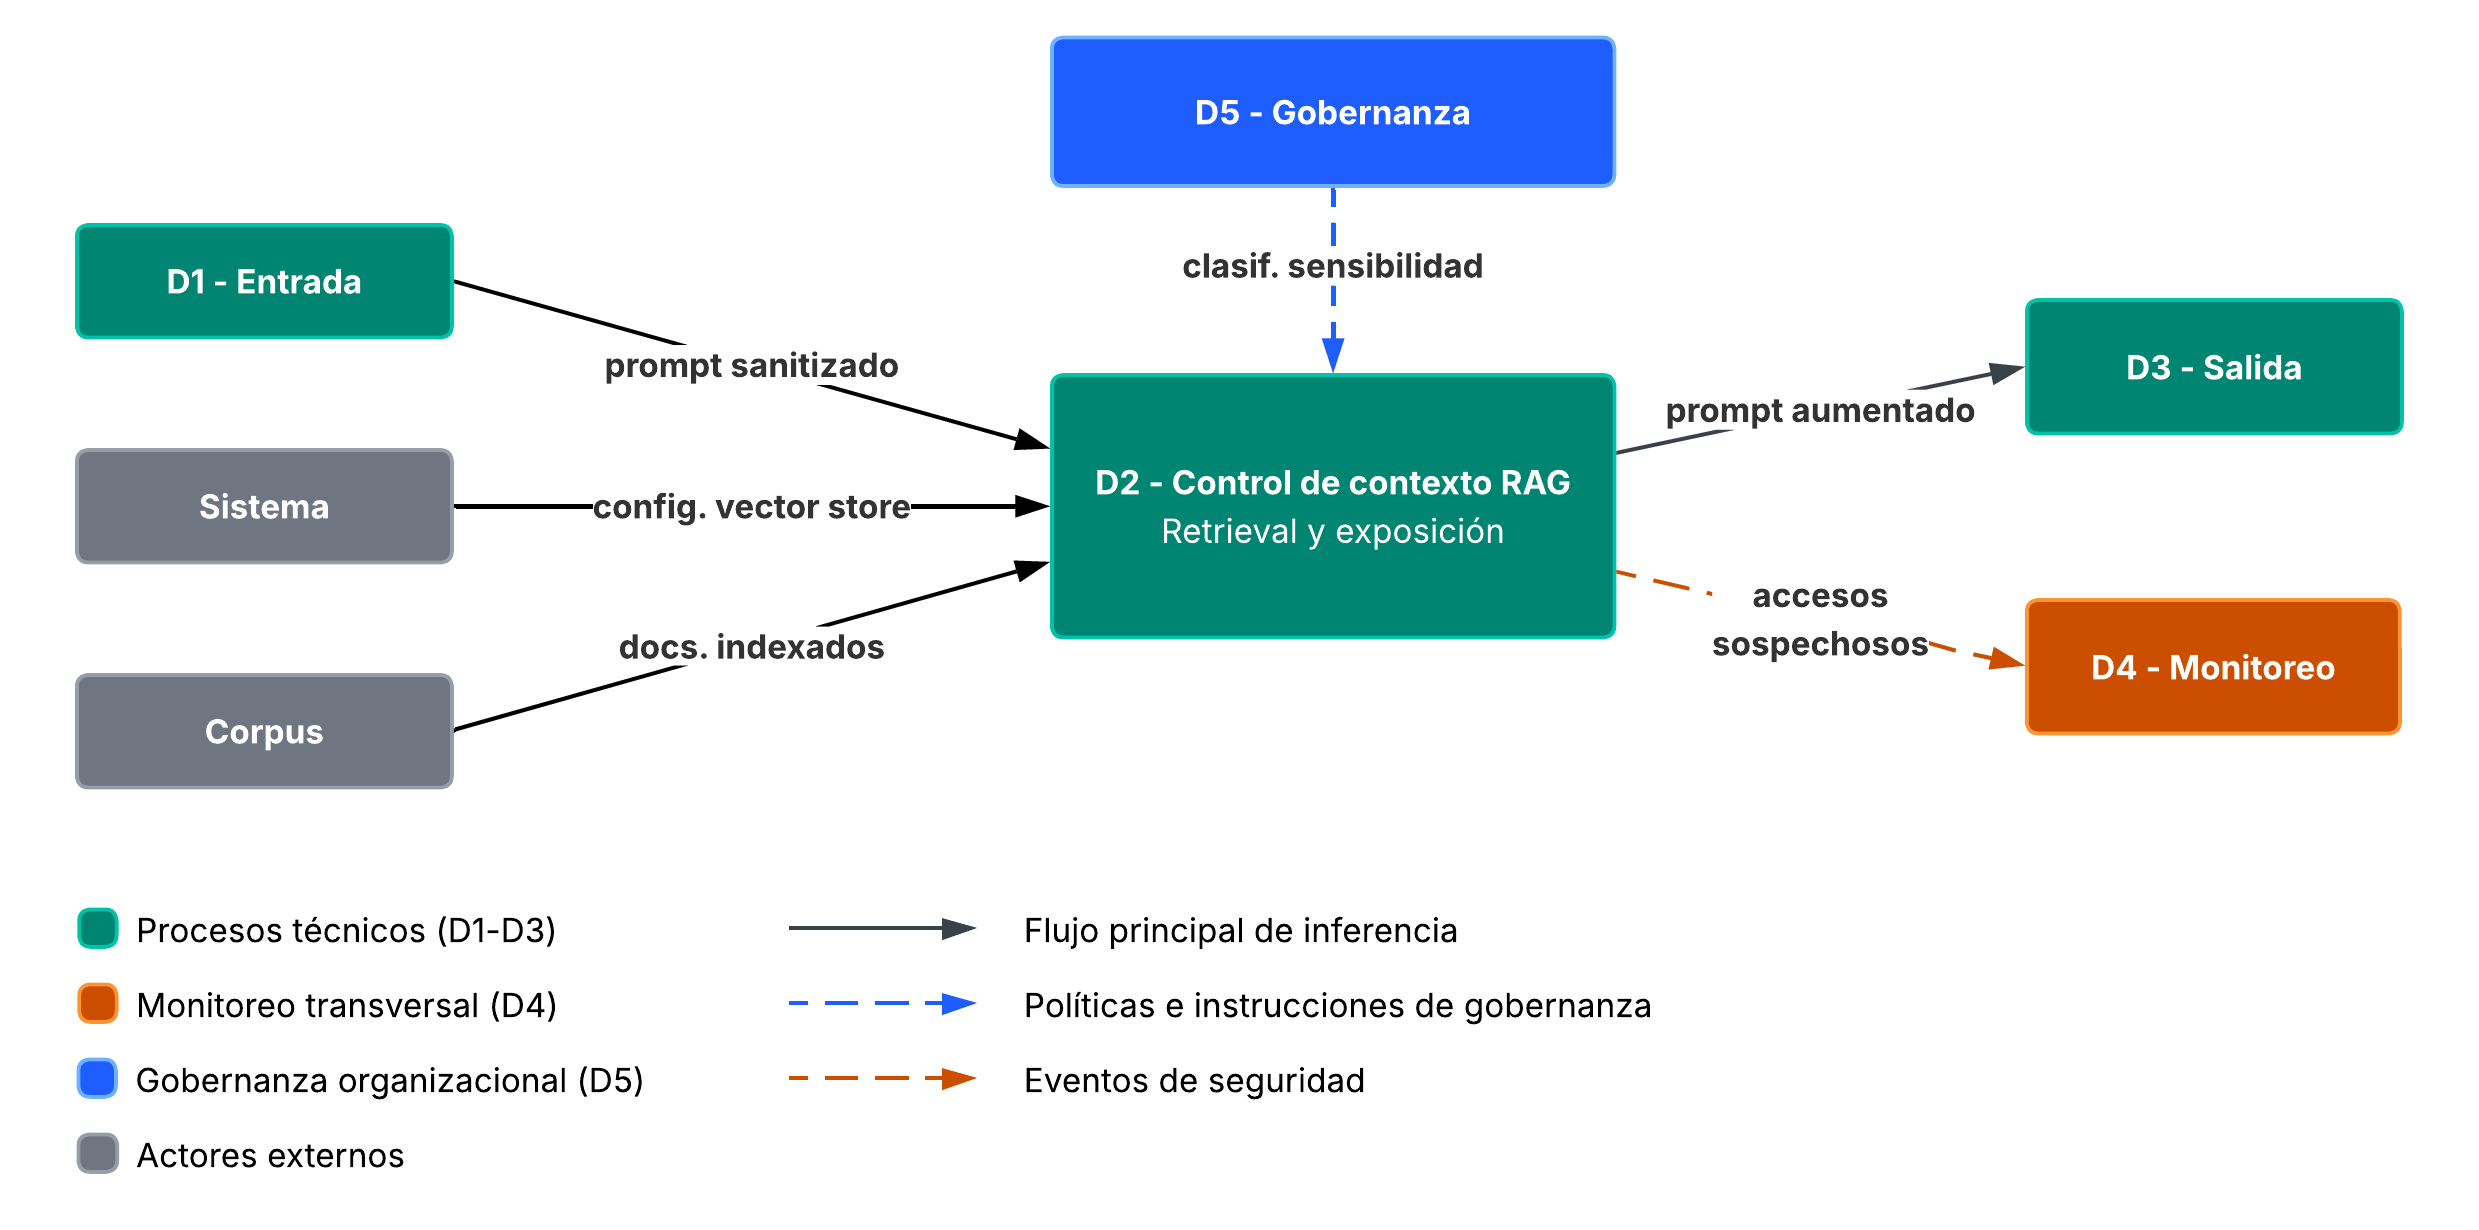
\includegraphics[width=0.95\linewidth]{figures/diagrama_D2.png}
    \caption{Flujo de entradas y salidas del proceso D2: Control de contexto y configuración RAG.}
    \label{fig:diagrama-d2}
\end{figure}

\subsection{D3: Gestión de salida}

La subdimensión D3 comprende los controles que filtran y regulan las respuestas generadas por el modelo antes de entregarlas al usuario. Opera sobre el canal de salida del flujo RAG, constituyendo la última línea de defensa contra la exfiltración de información sensible y la fuga del prompt del sistema.

La ficha del proceso y su especificación de entradas y salidas se presentan a continuación; la Figura~\ref{fig:diagrama-d3} representa gráficamente el mismo flujo.


\begin{fichabox}{Ficha del proceso D3: Gestión de salida}
  \begin{tabularx}{\textwidth}{@{} l X @{}}
    \textbf{Propósito} &
      Filtrar y controlar las respuestas generadas por el LLM, detectando y suprimiendo contenido sensible antes de que sea transmitido al usuario. \\[4pt]
    \textbf{Activos que protege} &
      Canales de salida y corpus de conocimiento. \\[4pt]
    \textbf{Vector OWASP asociado} &
      LLM02:2025, LLM07:2025 \\
  \end{tabularx}
\end{fichabox}

\begin{table}[H]
  \centering
  \caption{Entradas y salidas del proceso D3: Gestión de salida.}
  \label{tab:es-d3}
  \rowcolors{2}{llmsec-gray}{white}
  \begin{tabularx}{\textwidth}{@{} l >{\hsize=1.15\hsize\raggedright\arraybackslash}X >{\hsize=0.85\hsize\raggedright\arraybackslash}X l @{}}
    \toprule
    \textbf{Desde} & \textbf{Entrada} & \textbf{Salida} & \textbf{Hacia} \\
    \midrule
    D2 &
      Prompt aumentado con contexto recuperado &
      Respuesta sanitizada y validada &
      Usuario \\
    LLM &
      Respuesta generada &
      Registro de contenido suprimido &
      D4 \\
    Configuración &
      Patrones de detección de contenido sensible (YAML) &
      Alerta de fuga de información detectada &
      D4 \\
    D5 &
      Política de clasificación de sensibilidad &
      Registro de casos borde de clasificación no resueltos &
      D4 \\
    \bottomrule
  \end{tabularx}
\end{table}

\vspace{8pt}

\begin{figure}[H]
    \centering
    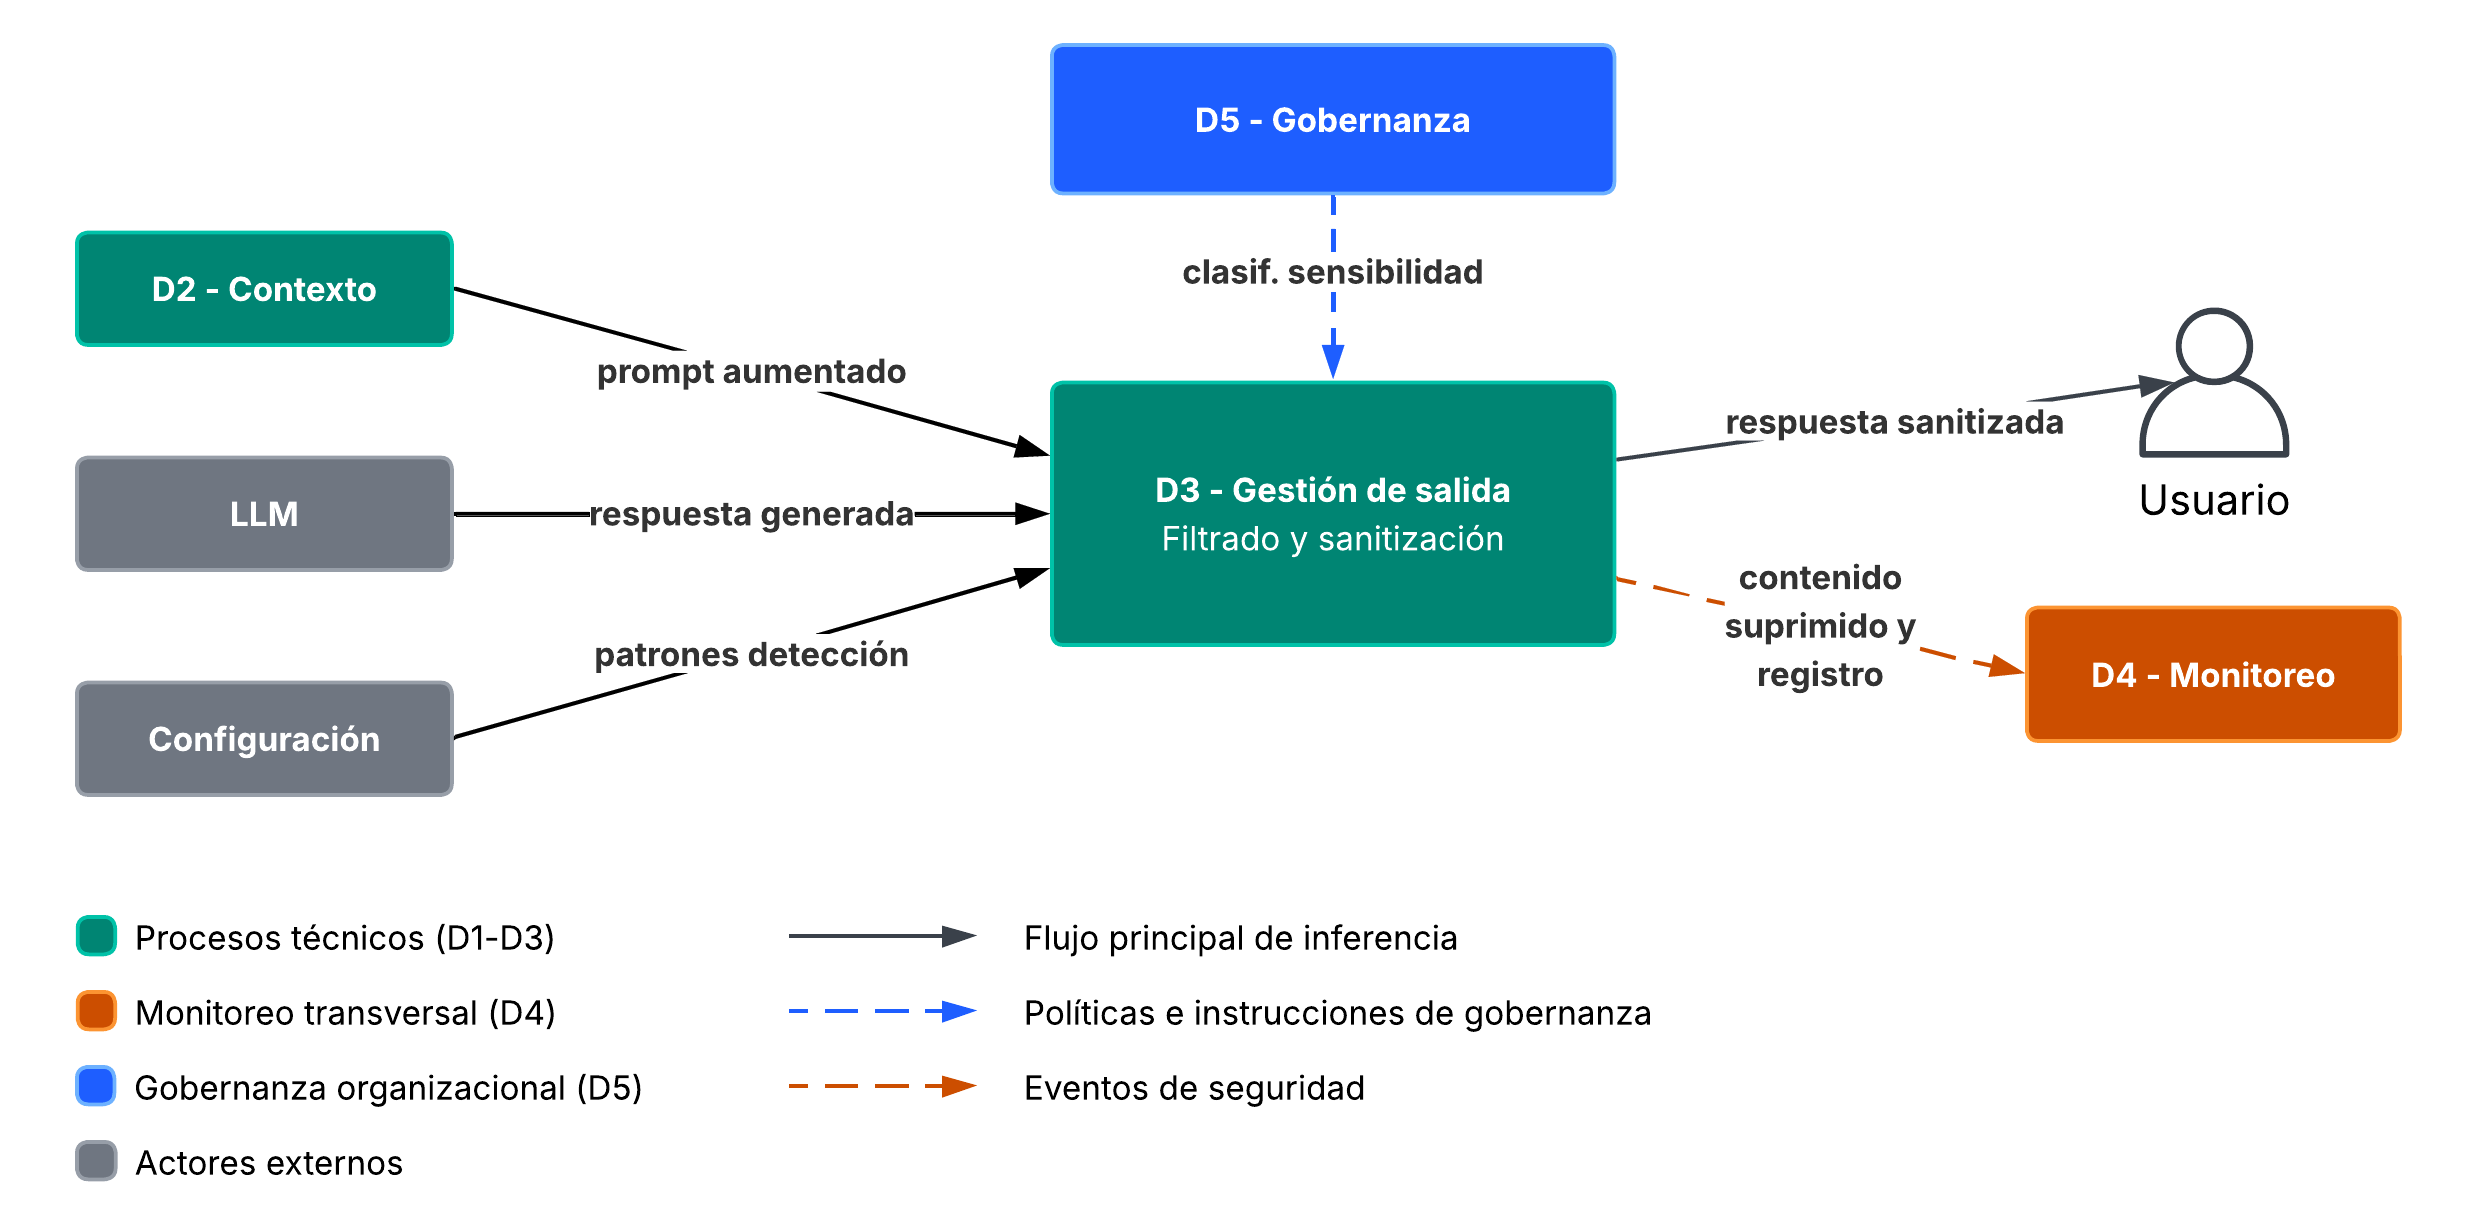
\includegraphics[width=0.95\linewidth]{figures/diagrama_D3.png}
    \caption{Flujo de entradas y salidas del proceso D3: Gestión de salida.}
    \label{fig:diagrama-d3}
\end{figure}

La política de clasificación de sensibilidad provista por D5 puede enfrentar casos borde: contenidos cuya clasificación no se resuelve de forma concluyente mediante los patrones y reglas definidos. Ante un caso borde, el proceso adopta un criterio conservador: el contenido se trata como sensible y se suprime de la respuesta. Adicionalmente, cada caso borde genera un registro específico hacia D4 para su monitoreo, de modo que la acumulación de casos no resueltos alimente la revisión de la política de clasificación en el ciclo de gobernanza, a través de la retroalimentación que D4 provee a D5.

\subsection{D4: Monitoreo y trazabilidad}

La subdimensión D4 opera de forma transversal sobre el sistema RAG completo. Su naturaleza es observacional: no interviene sobre el flujo sino que lo registra. Sus entradas son eventos generados por las tres subdimensiones anteriores y por el propio sistema, y sus salidas son artefactos de auditoría y de reporte.

Las entradas de D4 constituyen la telemetría del sistema: el conjunto de logs, eventos y métricas que los componentes del flujo RAG emiten durante su operación, incluyendo los registros de prompts rechazados (D1), los eventos de recuperación sospechosa (D2), los registros de contenido suprimido (D3) y las métricas de latencia del flujo de inferencia. Las alertas no constituyen un insumo independiente sino una consecuencia directa de esta telemetría: se generan cuando el monitoreo detecta, sobre los registros recibidos, condiciones que superan los umbrales definidos en la configuración de la capa defensiva. En consecuencia, la capacidad de alertamiento de D4 está acotada por la calidad y granularidad de la telemetría disponible.

Las salidas de D4 incluyen, además de los artefactos de auditoría, informes de desempeño y artefactos de visualización de métricas dirigidos a D5, donde se consolidan en los instrumentos de reporte hacia la dirección de la organización.

D4 no define controles de nivel N1 porque el monitoreo mínimo viable requiere que el sistema disponga de algún mecanismo activo de registro, condición que no se cumple en un sistema sin capa defensiva. Un sistema en esa condición se clasifica como no conforme en esta subdimensión.

La ficha del proceso y su especificación de entradas y salidas se presentan a continuación; la Figura~\ref{fig:diagrama-d4} representa gráficamente el mismo flujo.

\begin{fichabox}{Ficha del proceso D4: Monitoreo y trazabilidad}
  \begin{tabularx}{\textwidth}{@{} l X @{}}
    \textbf{Propósito} &
      Registrar, alertar y auditar los eventos de seguridad generados en el flujo RAG, garantizando trazabilidad completa sobre el comportamiento defensivo del sistema. \\[4pt]
    \textbf{Activos que protege} &
      Sistema RAG completo. \\[4pt]
    \textbf{Vector OWASP asociado} &
      LLM01:2025, LLM02:2025, LLM07:2025, LLM08:2025 \\
  \end{tabularx}
\end{fichabox}

\begin{table}[H]
  \centering
  \caption{Entradas y salidas del proceso D4: Monitoreo y trazabilidad.}
  \label{tab:es-d4}
  \rowcolors{2}{llmsec-gray}{white}
  \begin{tabularx}{\textwidth}{@{} l >{\hsize=1.20\hsize\raggedright\arraybackslash}X >{\hsize=0.80\hsize\raggedright\arraybackslash}X l @{}}
    \toprule
    \textbf{Desde} & \textbf{Entrada} & \textbf{Salida} & \textbf{Hacia} \\
    \midrule
    D1 &
      Registro de prompts rechazados y alertas de inyección &
      Logs de auditoría consolidados &
      D5 \\
    D2 &
      Eventos de recuperación sospechosa &
      Alertas de comportamiento anómalo &
      D5 \\
    D3 &
      Registro de contenido suprimido y alertas de fuga &
      Informe de incidentes de seguridad &
      D5 \\
    Sistema &
      Métricas de latencia del flujo de inferencia &
      Informes de desempeño y artefactos de visualización de métricas &
      D5 \\
    \bottomrule
  \end{tabularx}
\end{table}

\vspace{8pt}

\begin{figure}[H]
    \centering
    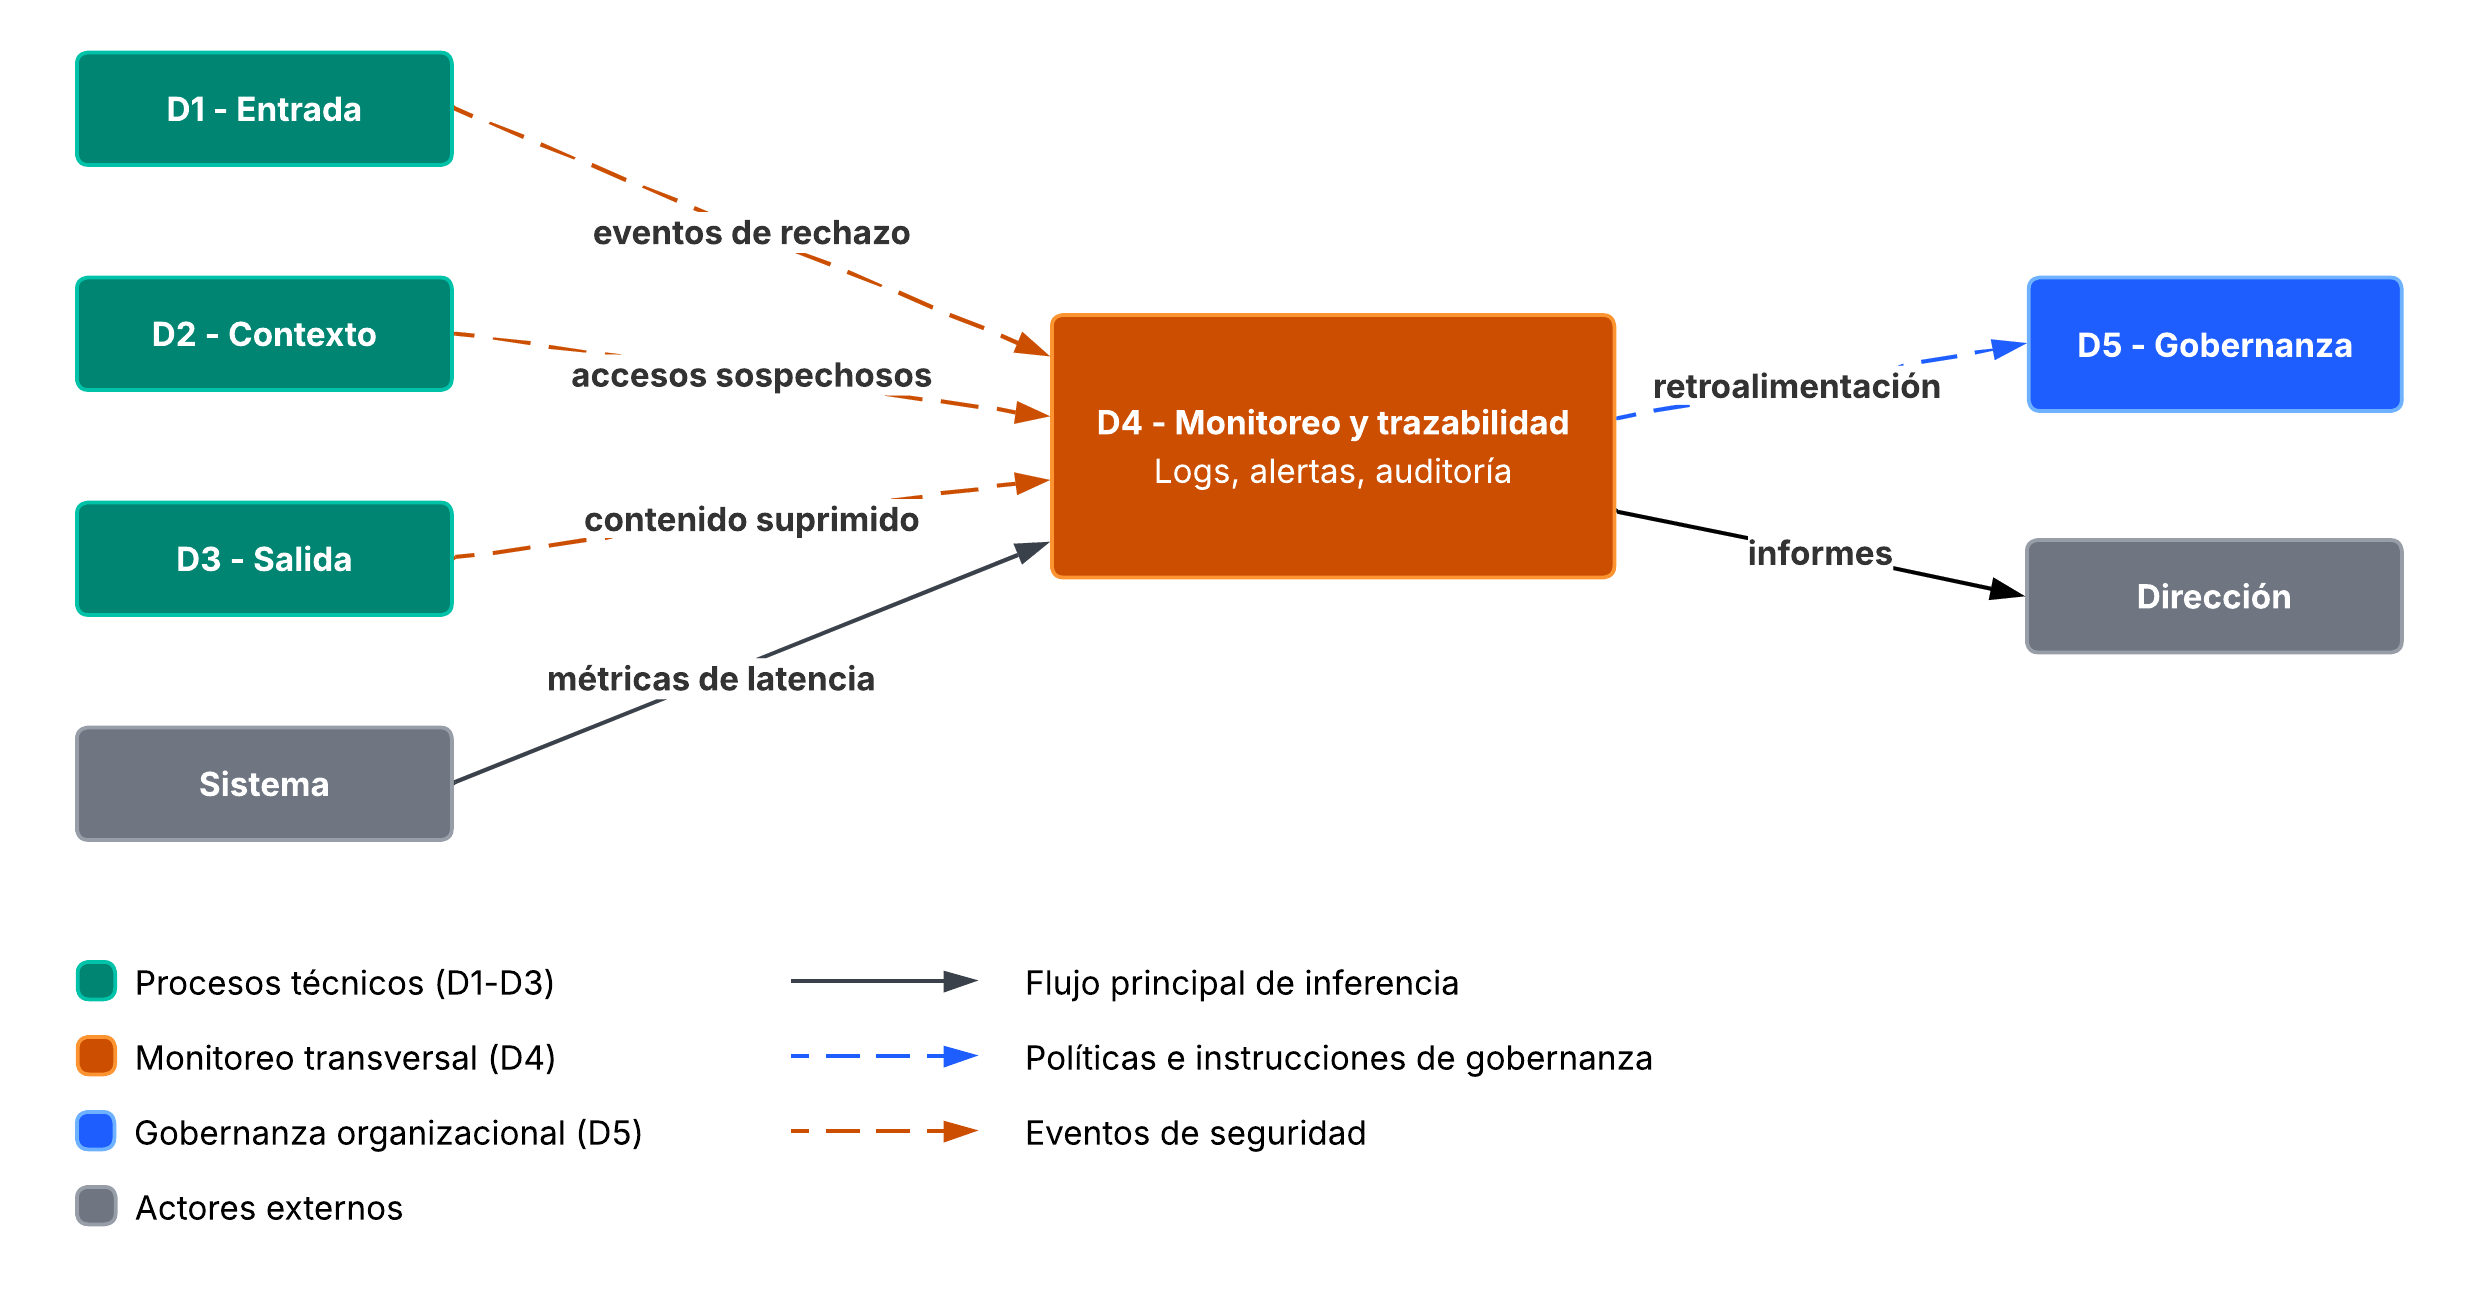
\includegraphics[width=0.95\linewidth]{figures/diagrama_D4.png}
    \caption{Flujo de entradas y salidas del proceso D4: Monitoreo y trazabilidad.}
    \label{fig:diagrama-d4}
\end{figure}

\subsection{D5: Gobernanza organizacional}

La subdimensión D5 opera de forma transversal sobre la organización completa, no sobre una etapa técnica específica del flujo RAG. Captura las obligaciones institucionales de gestión de la seguridad: definición de roles y responsabilidades, políticas de uso, cumplimiento normativo y mejora continua del marco. Su verificación es exclusivamente declarativa porque sus controles son artefactos organizacionales que no producen traza observable en el flujo de inferencia: su cumplimiento se establece mediante revisión documental y auditoría organizacional, no mediante inspección del sistema ni ejecución de pruebas ofensivas contra él.

D5 provee insumos normativos e institucionales a las demás subdimensiones, actuando como el proceso de gobernanza que sustenta la operación segura del sistema RAG en su conjunto. Sus entradas son marcos normativos y retroalimentación de D4, y sus salidas son políticas e instrumentos de gobernanza que condicionan la operación del resto del sistema.

La ficha del proceso y su especificación de entradas y salidas se presentan a continuación; la Figura~\ref{fig:diagrama-d5} representa gráficamente el mismo flujo.

\begin{fichabox}{Ficha del proceso D5: Gobernanza organizacional}
  \begin{tabularx}{\textwidth}{@{} l X @{}}
    \textbf{Propósito} &
      Establecer y mantener el marco institucional de gobernanza que sustenta la operación segura del sistema RAG, definiendo roles, políticas y mecanismos de mejora continua. \\[4pt]
    \textbf{Activos que protege} &
      Sistema RAG completo (a nivel organizacional) \\[4pt]
    \textbf{Vector OWASP asociado} &
      LLM01:2025, LLM02:2025, LLM07:2025, LLM08:2025 \\
  \end{tabularx}
\end{fichabox}

\begin{table}[H]
  \centering
  \caption{Entradas y salidas del proceso D5: Gobernanza organizacional.}
  \label{tab:es-d5}
  \rowcolors{2}{llmsec-gray}{white}
  \begin{tabularx}{\textwidth}{@{} l >{\hsize=1.10\hsize\raggedright\arraybackslash}X >{\hsize=0.90\hsize\raggedright\arraybackslash}X >{\raggedright\arraybackslash}p{2.2cm} @{}}
    \toprule
    \textbf{Desde} & \textbf{Entrada} & \textbf{Salida} & \textbf{Hacia} \\
    \midrule
    Normativa &
      Ley 21.663, Ley 21.719, Proyecto Ley IA &
      Política de uso aceptable &
      D1 \\
    NIST AI RMF &
      Marco de gestión de riesgos de IA &
      Política de clasificación de sensibilidad &
      D2 \\
    D4 &
      Logs de auditoría e informes de incidentes &
      Matriz RACI instanciada &
      D1--D4 \\
    D4 &
      Logs de auditoría e informes de incidentes &
      Informe de riesgos residuales &
      Dirección \\
    D4 &
      Logs de auditoría e informes de incidentes &
      Plan de capacitación en seguridad LLM &
      Roles definidos \\
    \bottomrule
  \end{tabularx}
\end{table}

\vspace{8pt}

\begin{figure}[H]
    \centering
    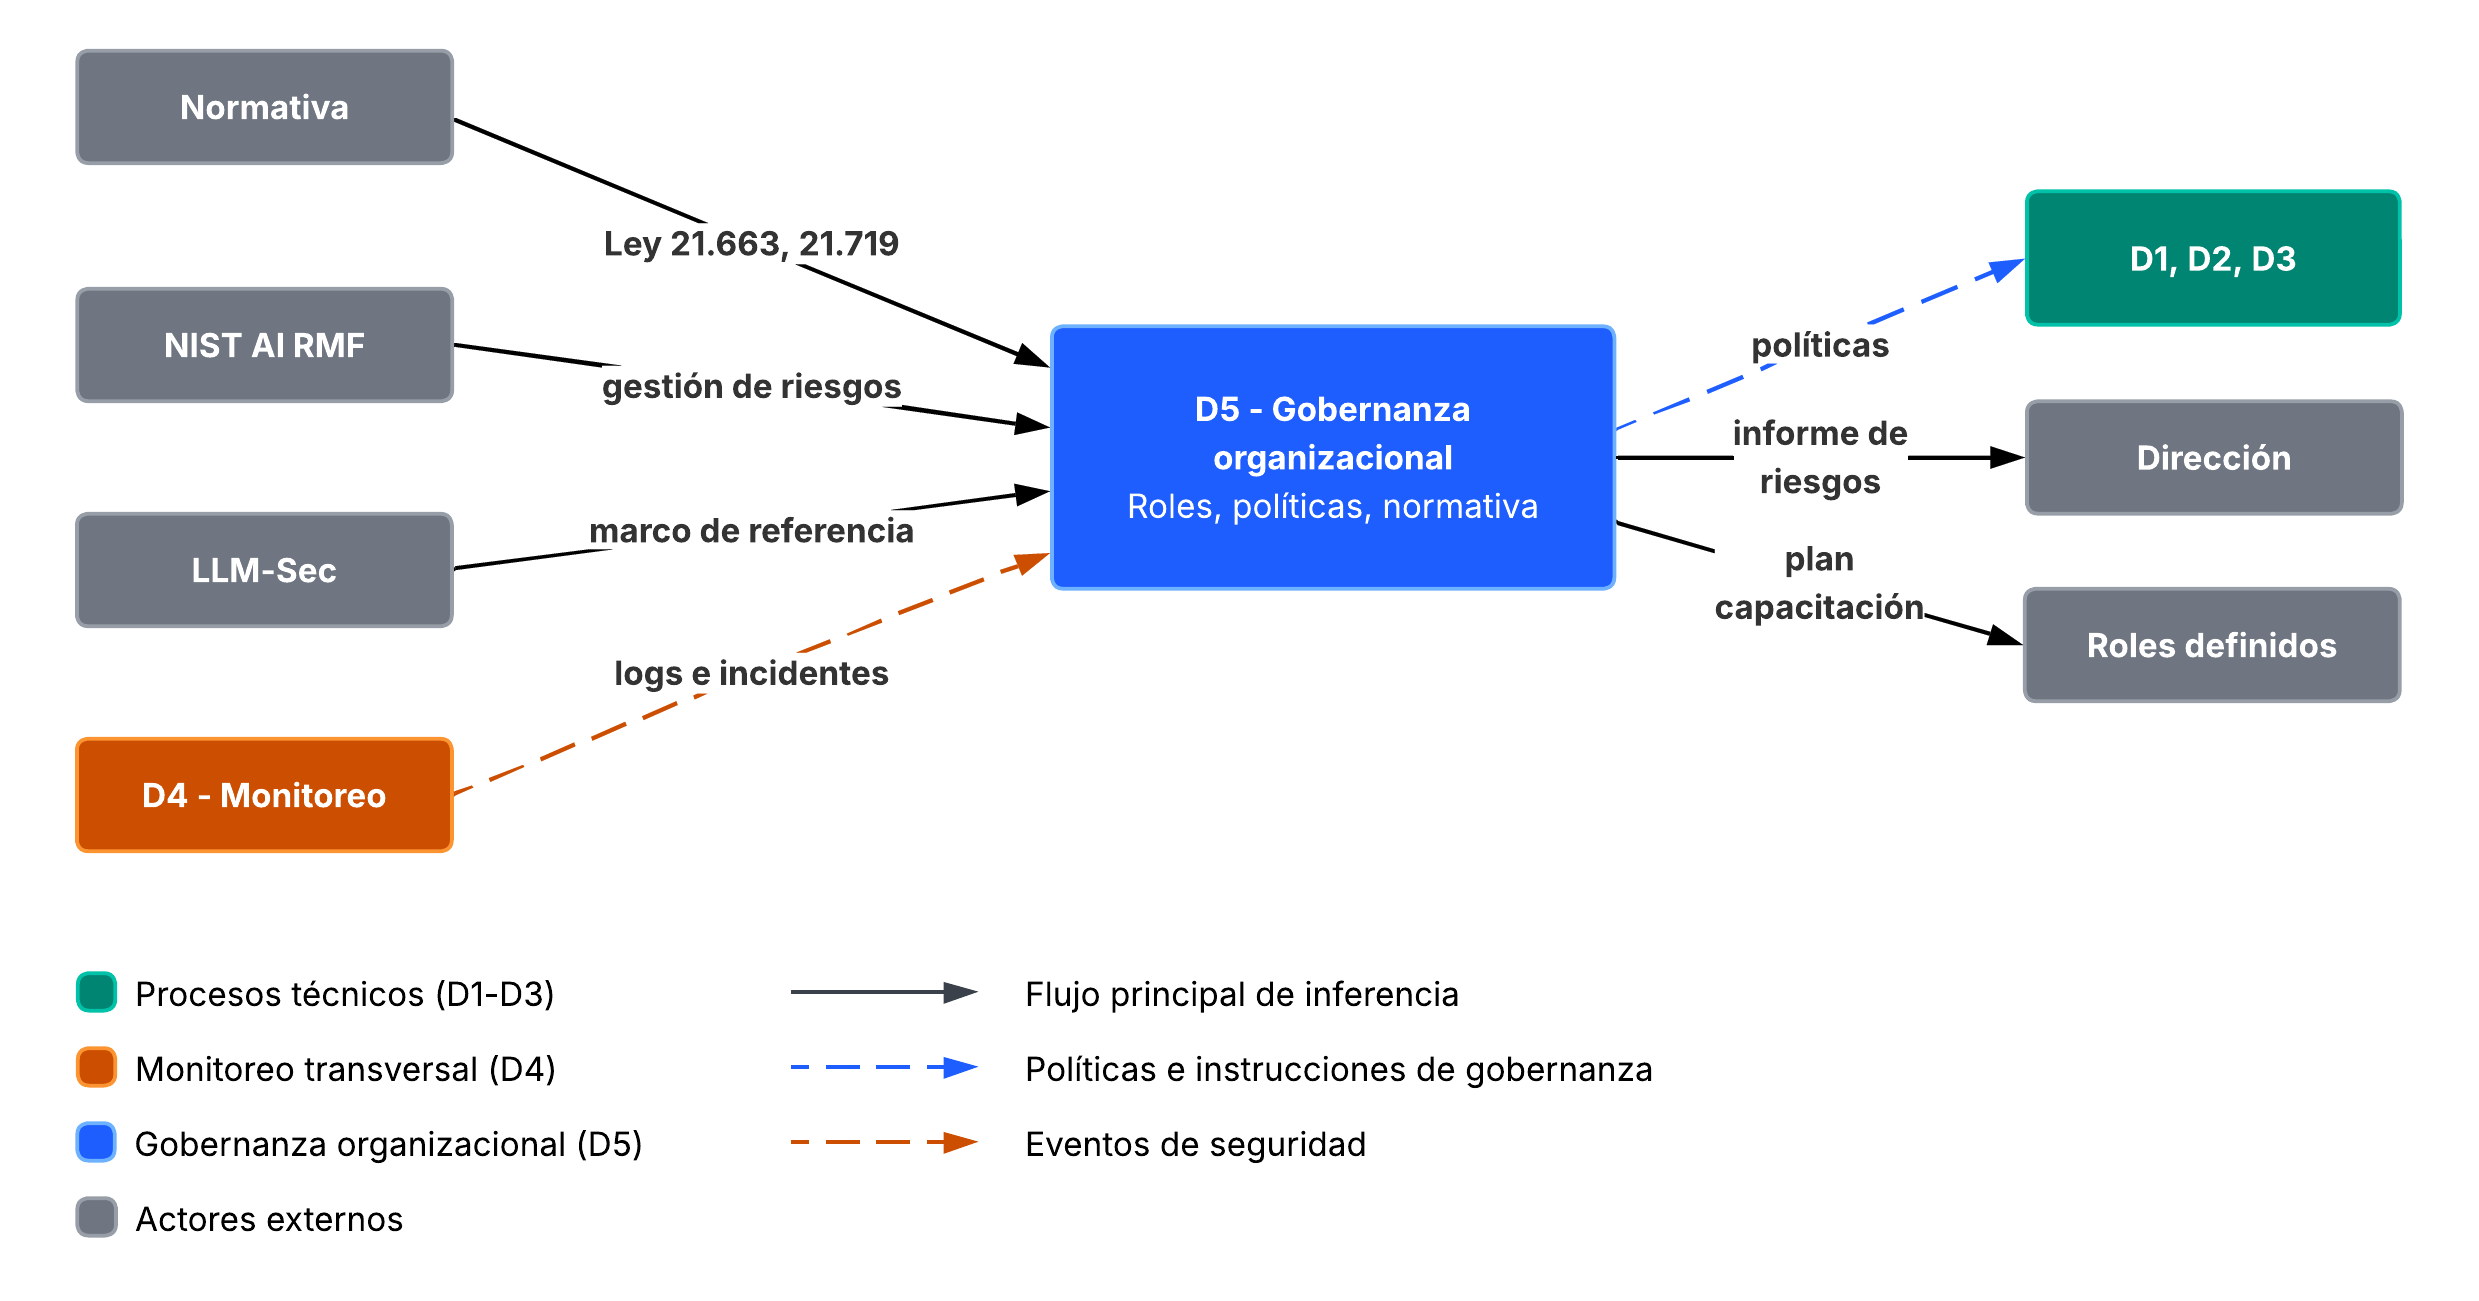
\includegraphics[width=0.95\linewidth]{figures/diagrama_D5.png}
    \caption{Flujo de entradas y salidas del proceso D5: Gobernanza organizacional.}
    \label{fig:diagrama-d5}
\end{figure}

\section{Nivel verificado y nivel declarado}
\label{sec:verificado-declarado}

Las subdimensiones del modelo no admiten el mismo tipo de evidencia. D1 a D4 operan sobre componentes técnicos del flujo RAG y su cumplimiento es constatable mediante inspección del sistema o ejecución de pruebas contra él. D5 captura obligaciones organizacionales que no producen traza técnica observable. El modelo distingue en consecuencia dos tipos de nivel asignado según la fuente de evidencia que lo sustenta:

\begin{infobox}
  \textbf{Nivel verificado:} determinado mediante evidencia experimental (resultados de auditoría ofensiva, logs de la capa defensiva) o de configuración (archivos YAML, prompt del sistema). Aplica a las subdimensiones D1, D2, D3 y D4.

  \textbf{Nivel declarado:} determinado mediante lista de chequeo sin evidencia técnica directa, basado en auditoría organizacional o revisión documental. Aplica a la subdimensión D5.
\end{infobox}

Esta distinción no establece una jerarquía entre ambos tipos de nivel: un control declarativo no es menos exigible que uno verificable, sino que su cumplimiento se constata por un medio distinto. La consecuencia práctica es que el nivel global de un sistema RAG no puede reportarse como un valor único sin especificar qué subdimensiones lo sustentan con evidencia técnica y cuáles con evidencia documental.

La dicotomía entre nivel verificado y nivel declarado describe la fuente de evidencia con que se acredita el cumplimiento de los controles, y es ortogonal a los constructos de agregación definidos en la sección~\ref{mad:constructos-agregacion}: el nivel técnico verificado agrega exclusivamente cumplimiento verificado en D1 a D4, el nivel de gobernanza $g$ corresponde al nivel declarado de D5, y el nivel integral combina ambas fuentes de evidencia en las cinco subdimensiones.

\section{Regla de piso mínimo}
\label{sec:piso-minimo}

El nivel global $L$ del sistema es el nivel integral definido en la sección~\ref{mad:constructos-agregacion}; en la notación introducida allí, $L = \min(d'_1, d'_2, d'_3, d'_4, g)$, donde $d'_i$ es el nivel de la subdimensión técnica $i$ sobre la totalidad de sus controles y $g$ es el nivel de gobernanza de D5, cuya fuente de evidencia es exclusivamente declarativa (sección~\ref{sec:verificado-declarado}). En consecuencia, el nivel global integra necesariamente una componente declarada, condición que debe hacerse explícita al reportar el resultado de la evaluación. La justificación subyacente es que la postura de seguridad de un sistema es tan sólida como su componente más débil. A modo de ejemplo, si D1, D2 y D3 alcanzan nivel 4, el nivel de gobernanza $g$ de D5 es 3 y D4 alcanza nivel 2, el nivel global es 2.

En cuanto a la ponderación dentro de cada subdimensión, todos los controles de un mismo nivel tienen peso equivalente. Esta decisión es consistente con la práctica de los modelos de madurez de la industria: OWASP SAMM \cite{owaspsamm} puntúa cada práctica de seguridad agregando las respuestas de evaluación sin pesos diferenciales entre actividades, y CMMI \cite{cmmi} no pondera prácticas individuales, sino que condiciona la consecución de un nivel a la satisfacción de la totalidad de las prácticas que lo componen, criterio análogo a la regla de progresión acumulativa y piso mínimo de LLM-Sec. La ausencia de literatura previa comparable sobre seguridad en arquitecturas RAG impide, adicionalmente, anclar ponderaciones diferenciales a evidencia empírica; asignar pesos arbitrarios introduciría un sesgo no justificable que los modelos de referencia tampoco asumen.

\subsection{Niveles de agregación: técnico verificado, de gobernanza e integral}
\label{mad:constructos-agregacion}

El marco distingue tres constructos de agregación según la fuente de evidencia que los sustenta, de modo que el alcance de cada afirmación de nivel quede acotado a la evidencia que efectivamente la respalda.

El nivel técnico verificado agrega las subdimensiones D1 a D4 considerando exclusivamente los controles de fuente experimental o de configuración:
\begin{equation}
L_{\text{tec}} = \min(d_1, d_2, d_3, d_4)
\end{equation}
donde $d_i$ es el mayor nivel de la subdimensión $i$ cuyos controles verificables están completamente implementados, respetando la progresión acumulativa. Este constructo corresponde a la evidencia que un entorno de laboratorio controlado puede producir.

El nivel de gobernanza $g$ corresponde al nivel alcanzado por la subdimensión D5, cuya fuente de evidencia es exclusivamente declarativa y se acredita mediante auditoría documental o entrevistas, conforme a la sección~\ref{sec:crit-declarativo}.

El nivel integral agrega ambos constructos e incorpora los controles declarativos de las subdimensiones técnicas:
\begin{equation}
L = \min(d'_1, d'_2, d'_3, d'_4, g)
\end{equation}
donde $d'_i$ se calcula sobre la totalidad de los controles de la subdimensión $i$, incluidos los de fuente declarativa. El nivel integral solo es calculable cuando la organización ha realizado la auditoría declarativa correspondiente. En su ausencia, el marco reporta el nivel técnico verificado y declara el nivel integral como no evaluado. Un nivel integral no evaluado no debe asimilarse a N0: la no conformidad expresa incumplimiento constatado, mientras que la no evaluación expresa ausencia de medición.

\subsection{Alcanzabilidad del nivel global N1}
\label{mad:alcanzabilidad-n1}

La subdimensión D4 no define controles de nivel N1: el monitoreo mínimo viable de un sistema LLM exige la presencia de al menos un componente activo de registro de eventos, condición que no se satisface sin una capa defensiva implementada. En consecuencia, el menor nivel activo alcanzable por D4 es N2 y, por aplicación de la regla de piso mínimo, la imagen de la función de agregación global es $\{N0, N2, N3, N4, N5\}$: el nivel global N1 no es alcanzable por construcción.

Esta asimetría es una decisión de diseño deliberada y no un defecto de la regla de agregación: un sistema que carece de todo mecanismo de monitoreo no puede considerarse globalmente maduro en grado alguno, aun cuando sus etapas individuales del flujo RAG satisfagan condiciones mínimas de higiene. El carácter ordinal y acumulativo del modelo se preserva íntegramente al interior de cada subdimensión, y el nivel N1 conserva su semántica como nivel alcanzable en las subdimensiones D1, D2, D3 y D5, conforme a la distribución de la Tabla~\ref{tab:distribucion-controles}.